%!TEX root = ../main.tex

\chapter{Introduction} \label{ch:Intro}
Over the past decades, air traffic has increased rapidly, leading to a global increase in CO$_2$ emissions along with other green-house gases. This emission increase can be locally slowed down by replacing old aircrafts with newer models \cite{emission}, but unfortunately only temporary, as all air traffic forecasts point to a rapid growth \cite{airbus,jadc}. To make flight more sustainable over a longer period, continuous performance improvements are needed. One major aspect in improving the aircraft performance is to increase the aircraft engine efficiency.

The improvement of the engine efficiency has been quite successful over the past decades, specially with the increased usage of Computational Fluid Dynamics (CFD). This has led to the development of the high bypass-ratio turbo-fan engines with large fans and high pressure-ratio engine cores, as it combines the relatively high efficiency, high sub-sonic aircraft velocities and low noise levels. Further efficiency improvements are however getting harder to achieve with current methodologies. In the design process the engine components are usually divided into several modules, where each module is optimized separately with simplified interaction. Ghisu et al. \cite{IntegrP2} showed that optimizing components isolated from each other could result in sub-optimal designs. The sub-optimal designs can unfortunately lead to expensive redesigns late in the design process. However, by including more components in a single design process, the risk can be lowered substantially. This integrated design process takes the advantages of lowering the need for simplified or modeled interaction between components, resulting in a more optimal solution earlier in the design process \cite{IntegrP1,IntegrP2}.

\section{The aircraft engine\label{ch:engine}}
%\ignore{Citation missing: Boundary condition effects - 1}
%Describe a turbofan engine\\
A modern high bypass-ratio turbo-fan engine, like the one presented in Figure \ref{fig:engine}, consists of six major aerodynamic components. The fan, which is located at the engine inlet, accelerates the air where a fraction goes into the engine core whereas most of the air is bypassed. The bypassed air is responsible for most of the engine's thrust. Typically, newer high bypass-ratio turbo-fan engines have a bypass ratio of 8-12. Downstream of the fan the engine's core flow enters the low-pressure compressor (LPC), followed by the high-pressure compressor (HPC), where the first and second stages of compressions are performed, respectively. Downstream of the HPC the flow is directed into the combustion chamber (CC) and the high and low pressure turbines (HPT and LPT, respectively). In the CC the fuel is injected into the compressed air and ignited to increase the energy of the fuel-air mixture. In the HPT, energy is extracted from the core flow to drive the HPC whereas the LPT, for a two-spool engine configuration, drives both the LPC and the fan. For a three-spool configuration, the LPT is divided into two components, where each component drives separate shafts to obtain different rotational speeds for the fan and the LPC. For the two-spool configuration, the different rotational speed is obtained by using a geared shaft.

\begin{figure}[H]
%Turbofan: https://www.aviationcv.com/aviation-blog/2016/worlds-biggest-jet-engine-first-testing
  %Borja had this reference: http://pw.utc.com/
    \centering
  \begin{tikzpicture}
    \node[anchor=south west,inner sep=0] at (0,0) {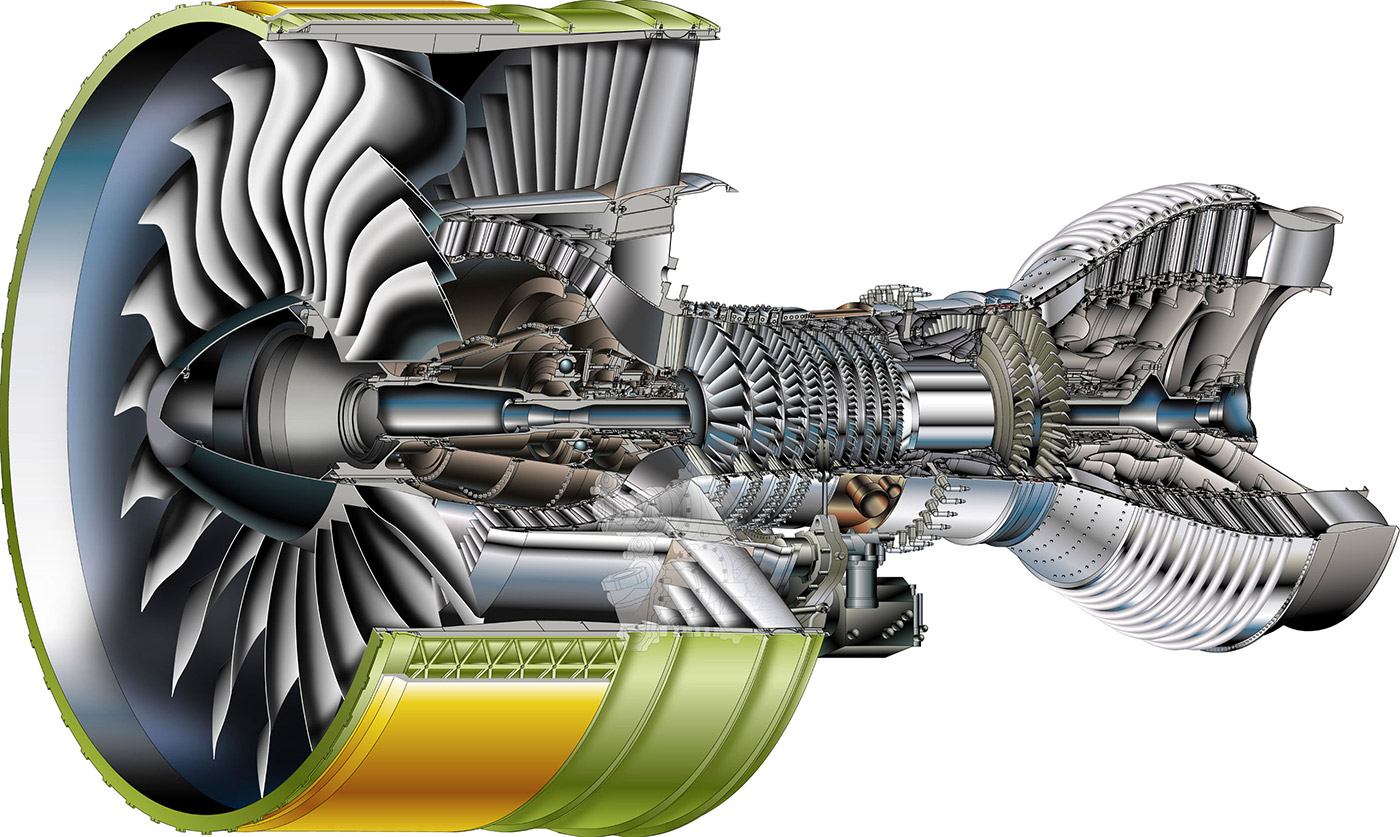
\includegraphics[width=0.7\linewidth]{figures/ge9x.jpg}};
    %\draw[help lines,step=.2] (0,0) grid (10,7);
    \node at (1.05,6.3) {\bf{Fan}};
    \draw[-latex,thick, red] (1.05,6.1)--(1.7,4.6); %-0.15,-0.5
    \node at (3.65,6.3) {\bf{LPC}};
    \draw[-latex,thick, red] (3.65,6.1)--(3.8,4.);
    \node at (5.4,5.0) {\bf{ICD}};
    \draw[-latex,thick, red] (5.4,4.8)--(4.3,3.6); %-0.4,-0.2
    \node at (5.8,4.3) {\bf{HPC}};
    \draw[-latex,thick, red] (5.8,4.1)--(5.4,3.3); %-0.6,-0.3
    \node at (6.5,4.85) {\bf{CC}};
    \draw[-latex,thick, red] (6.5,4.65)--(6.4,3.45); %-0.7,-0.35
    \node at (7.3,5.6) {\bf{HPT}};
    \draw[-latex,thick, red] (7.3,5.4)--(6.9,3.4);%-0.7,-0.4
    \node at (8.6,5.2) {\bf{LPC}};
    \draw[-latex,thick, red] (8.6,5.0)--(8.2,4.0); %-0.4,-0.2


  \end{tikzpicture}
  \caption{The two spool GP7000 turbofan engine \cite{GP7000}.}\label{fig:engine}
\end{figure}\noindent

One component of the engine that has gotten less interest over the years, compared to the already mentioned components, with the respect to performance analysis and improvements, is the S-shaped intermediate compressor duct (ICD). The ICD is located in between the LPC and HPC and is designed to guide the flow from the larger radius LPC towards the HPC. The LPC tends to have larger hub-to-tip radius for more efficient compression whereas the HPC has lower radius to limit the tip leakage losses and reduce the disk weight. This means that the ICD must force the flow through the S-shaped annular duct over a large radial offset to achieve a more efficient engine. Furthermore, the radial offset should be done in as short axial distance as possible to limit the size and weight of the engine, resulting in aggressive duct design. If the forcing is however done to aggressively the flow might separate at the convex inner wall, due to strong adverse pressure gradient. There exist few studies where the aim was to analyse the performance of an S-shaped duct. Britchford et al. \cite{Britchford1994} analysed the flow field of a clean S-shaped duct. The conclusion from the study was that the flow inside such a duct is complex and influenced by strong curvature and stream wise pressure gradient with high risk of separation at the inner wall. In another study by Britchford et al. \cite{Britchford1994b}, an upstream rotor was found to be an efficient way to re-energize the boundary layer at the inner wall, decreasing the adverse pressure gradient, resulting in lower risk of separation. Bailey et al. \cite{Bailey} showed that the pressure losses of a clean S-shaped duct with well-behaved flow and without separation were comparable to a parallel sided duct despite the strong curvature and pressure gradient effects. Furthermore, they showed that by introducing the strut (described later), the pressure losses were increased due to increased blockage, resulting in thicker boundary layers at the inner and outer casings. Karakasis et al. \cite{Karakasis2010} studied the performance of an axisymmetric and non-axisymmetric ducts, where experimental data was compared to CFD with good results for the flow close to the inner casing but could however not capture the structure accurately at the outer wall. The study also gave a good description of the mechanics in an ICD with a strut and upstream compressor.

Figure \ref{fig:enginezoom} shows a zoom in on the ICD of the engine presented in Figure \ref{fig:engine}. The rear stages of the upstream LPC and first stages of the downstream HPC can be seen as well as the radial offset between the two. To analyse the flow physics of the ICD in details, an experimental rig has been built at GKN Aerospace in Trollh\"{a}ttan, Sweden. The experimental rig represents a simplified ICD were the strut, upstream guide vanes and a representative of the last rotating blade row (rotor) of the upstream LPC is included. Figure \ref{fig:schema} illustrates how the test section of the experimental rig is set up. It consists of pre-swirlers (PSW), bleed pipe, outlet guide vanes (OGV) and struts, where all but the PSW represent a real engine component. The PSW, which is a stationary blade row, is located upstream of the test section to replicate rotor exit-flow from the rear stage of a real engine compressor. Using stationary blades results in simpler simulations, saving computational resources. The bleed pipe represents the passage where bleed flow is extracted from the main flow to ensure stable compressor operation at part-speed. The OGV:s are placed downstream of the bleed pipe to guide the flow correctly into the ICD. The OGV:s are integrated into the ICD to achieve shorter length \cite{Walker2011}, with lower risk of separation and designed to minimize the upstream effects of the strut's potential field. The strut, which has a zero-lift wing profile, is located inside the duct to add mechanical strengthening as well as provide services to the engine core in terms of oil and electrical pipes, but as disused before, increases the losses as well as the complexity of the flow structures in the ICD.
\begin{figure}[H]
  \centering
  \begin{tikzpicture}
    \node[anchor=south west,inner sep=0] at (0,0) {  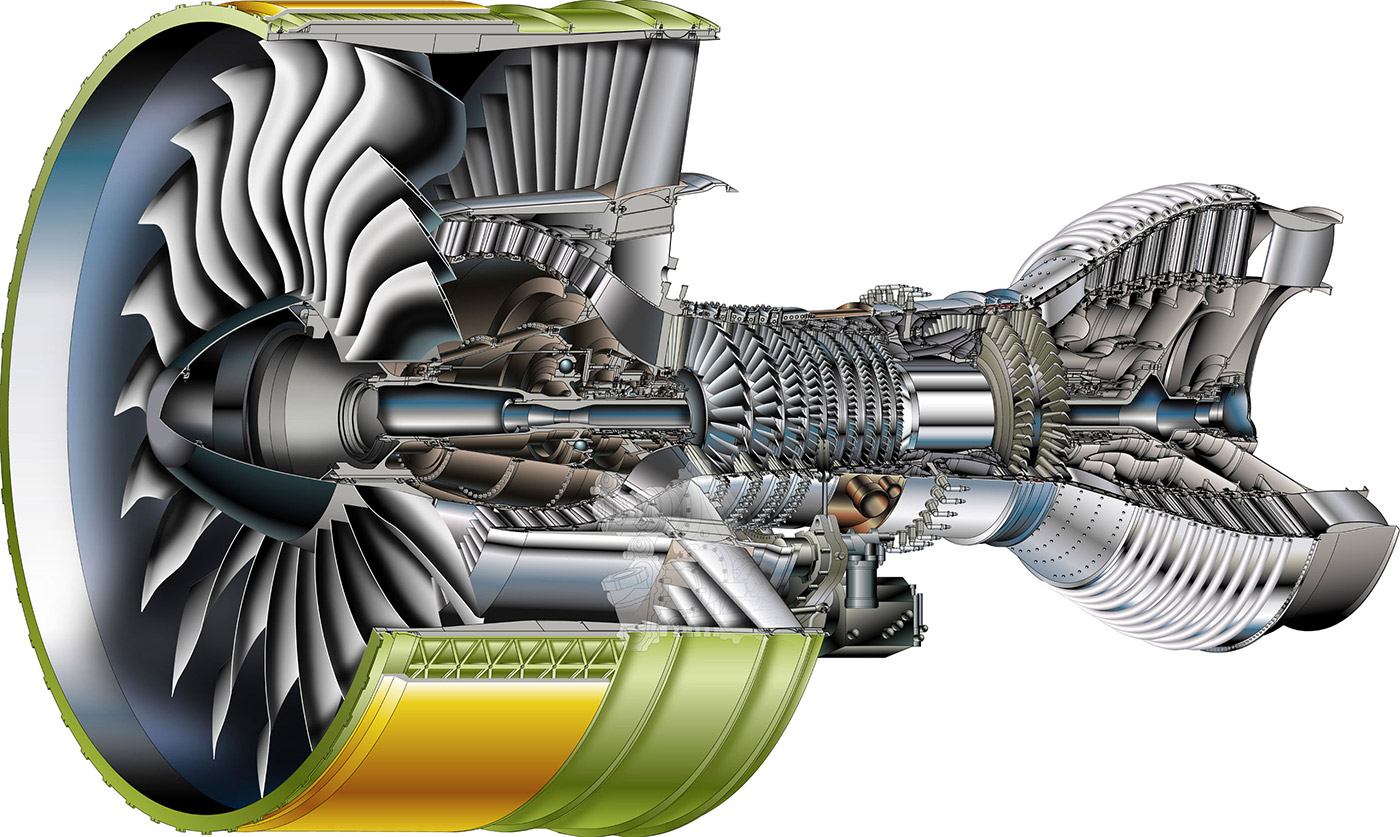
\includegraphics[width=0.5\linewidth, trim=19cm 15cm 22cm 9cm, clip]{figures/ge9x.jpg}};
    \node at (3,4.2) {{\color{red}\bf{Strut}}};
    \draw[-latex,thick, red] (3,4.0)--(2.4,3.2);
    \node at (0.9,3.0) {{\color{red}\bf{OGV}}};
    \draw[-latex,thick, red] (0.9,3.2)--(1.4,4.0);
    \node at (5.6,4.2) {{\color{red}\bf{HPC}}};
    \draw[-latex,thick, red] (5.6,4.)--(5.2,2.2);
    %\draw[help lines,step=.2] (0,0) grid (7,5);
  \end{tikzpicture}
\caption{Zoom in on the ICD, including the last stages of the LPC and first stages of the HPC.} \label{fig:enginezoom}
\end{figure}

Generally, there are 8-10 struts in an aircraft engine and the number of OGV:s are usually an order of magnitude higher than the number of struts. To permit the use of the same tangential sector for all domains in CFD simulations without having to include the full cross-section of the duct, the experimental rig was set up with 9 struts and 81 OGV:s. The same was done for the PSW, which has 45 blades in total.

 \begin{figure}[h!]
   \centering
%\documentclass[12pt,english]{article}
%\usepackage{fullpage}
%\usepackage[T1]{fontenc} 
%\usepackage{helvet}
%\renewcommand{\familydefault}{\sfdefault}
%\usepackage{babel}
%\usepackage{amsmath}
%\numberwithin{equation}{section}
%\usepackage{hyperref}
%\usepackage{tikz,pgfplots}
%\usepackage{boldline} %To get thicker lines in tables
%\usepackage{float}    %For float on figures for exampel
%\usepackage{graphicx} %Figures
%
%\usepackage{sectsty}
%\allsectionsfont{\centering}
%
%\renewcommand{\thesubsection}{\Roman{subsection}} 
%\renewcommand{\thesubsubsection}{\Alph{subsubsection}} 
%
%\newcommand{\ignore}[1]{}
%
%\begin{document}
%
%\begin{figure}[H]
%  \centering
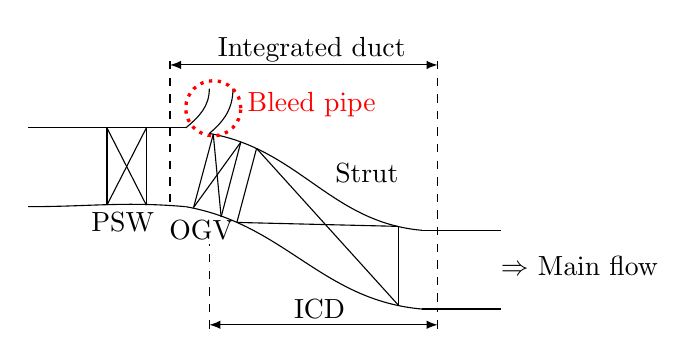
\begin{tikzpicture}
  \coordinate (A) at (-1,1);
  \coordinate (B) at (1,1);
  \coordinate (C) at (1.3,1.5);
  \coordinate (D) at (1.6,1.5);
  \coordinate (E) at (1.3,0.93);
  \coordinate (F) at (4,-0.3);
  \coordinate (G) at (5,-0.3);
  \coordinate (H) at (-1,0);
  \coordinate (I) at (1,0);
  \coordinate (J) at (4,-1.3);
  \coordinate (K) at (5,-1.3);
  %Upper side
  \draw (A)--(B);
  \path [black,out=40,in=-90] (B) edge (C);
  \path [black,out=-90,in=40] (D) edge (E);
  \path [black,out=-10,in=175] (E) edge (F);
  \draw (F)--(G);
  \draw[red,dotted, very thick] (1.35,1.25) circle (0.35);
  \node[red] at ([shift={(1.0,-0.2)}]D) {Bleed pipe};
  %Lower side
  \path [black,out=0,in=175] (H) edge (I);
  \path [black,out=-10,in=175] (I) edge (J);
  \path [black,out=0,in=180] (J) edge (K);
  %PSW
  \draw (0,1)--(0,0.02);
  \draw (0.5,1)--(0.5,0.02);
  \draw (0,0.02)--(0.5,1.0);
  \draw (0.5,0.02) -- (0,1);
  %\node at ([shift={(1.2,0.2)}]A) {PSW};
  %OGV
  \draw (1.35,0.92) -- (1.1,-0.01);
  \draw (1.7,0.82) -- (1.45,-0.13);
  \draw (1.35,0.92) -- (1.45,-0.13);
  \draw (1.7,0.82) -- (1.1,-0.01);
  %\node at ([shift={(0.0,-0.3)}]I) {OGV};
  %Duct
  \draw (1.9,0.74) -- (1.65,-0.2);
  \draw (3.7,-0.25) -- (3.7,-1.25);
  \draw (1.9,0.74) -- (3.7,-1.25);
  \draw (3.7,-0.25) -- (1.65,-0.2);
  %\node at ([shift={(1.8,-0.5)}]E) {Duct};

  %Marking the Integrated duct
  \node at ([shift={(1.0,0.5)}]D) {Integrated duct};
  \draw[latex-latex] (0.8,1.8)--(4.2,1.8);
  \draw[dashed] (0.8,1.85)--(0.8,0);
  \draw[dashed] (4.2,1.85)--(4.2,-1.3);
  %Marking the duct
  \node at ([shift={(-1.3,0.)}]J) {ICD};
  \draw[latex-latex] (1.3,-1.5)--(4.2,-1.5);
  \draw[dashed] (1.3,-1.55)--(1.3,-0.48);
  \draw[dashed] (4.2,-1.55)--(4.2,-1.3);

  %Mark Front Traverse surface
  %\draw[dashed, thick] (0.8,1.2)--(0.8,0);
  %Strut
  \node at ([shift={(2.0,-0.5)}]E) {Strut};
  %PSW
  \node at ([shift={(1.2,-0.2)}]H) {PSW};
  %OGV
  \node at ([shift={(0.2,-0.3)}]I) {OGV};
  %Main flow
  \node at ([shift={(1.0,-0.45)}]G) {$\Rightarrow$ Main flow};
\end{tikzpicture}
%  \caption{Schematic of the integrated compressor duct design}
%  \label{fig:schema}
%\end{figure}
%\end{document}

  \caption{Schematic of the integrated compressor duct design.}
  \label{fig:schema}
\end{figure}
%flow field of ICD, Cambridge references. schematic figure\\

Designing an ICD lacks practical design rules and therefore a combination of CFD and optimization is usually applied. The ICD has not been optimized to the same extent as surrounding components. Still, there have been some successful studies where the objective was to optimize or analyse the ICD \cite{CompressorOpt,OptComp1,OptComp2,Walker2011}, resulting in shorter and lighter engines, with more aggressive flow guidance. The interaction between the duct and the surrounding components has, however, not been addressed in the same way, even though it has been showed that it can improve the performance substantially \cite{IntegrP2}. If not considered, this isolation can result in a limited design space for the optimization, as the internal flow field of the duct is highly dependent on the surrounding components. For that reason, a more integrated design approach should be considered early in the design process.

One constraint, in applying a more integrated design approach is computational resources, as including more components results in higher computational demand. That demand even increases further when 3D CFD simulations are considered. Furthermore, to be able to take full advantages of the CFD simulation and the integrated design, a step towards Large Eddy Simulation (LES) needs to be taken to get a better idea of flow separation and complicated flow behaviour that is not captured to the same extent by the more common Reynolds Averaged Navier-Stokes (RANS) models. In this thesis, to limit the computational cost to some extent, the hybrid LES/RANS model Delayed Detached Eddy Simulation (DDES), introduced by Spalart et al. \cite{DDES}, is used as it combines the abilities of the LES in resolving the transient flow features of the main flow and the RANS models in calculating the attached near wall behaviour with reasonable grid density. 

%The original DES model was introduced by Spalart et al. \cite{DES97} as a hybrid between LES and RANS turbulence models based on the Spalart-Allmaras (SA) one equation model \cite{SA}. Initially the model was only presented for a 2D application but extended to 3D by Shur et al. \cite{DES99}. In that study, the performance of the DES model gave a promising result which lead to a wide usage. It was however shown that for grids with stream-wise grid spacing of similar size as the boundary layer a premature switching from RANS to LES could happen. This was the motivation for the new and improved DES, called Delayed DES (DDES) \cite{DDES}. In the DDES model the switching between RANS and LES is no longer governed only by the grid density but also the solution itself. This has greatly improved the application of the model as less time can be spent in generating satisfactory grids. \\
\section{Aim}
The initial objective was to analyse the flow-physics of the ICD by applying models of higher fidelity. This is expected to give better understanding of the complicated flow features presented in the ICD, especially when considering the effects from the bleed pipe. As this was more time-consuming than anticipated due to complex implementations, the initial step is limited to more simplified modelling techniques. First step is to apply more common and less computationally demanding RANS models (Chapter \ref{ch:sim}).

Secondary objective of this thesis is to evaluate the performance of an in-house code in uncharted areas. This will give valuable feedback where improvements are needed, resulting in more competitive solver.

%Initial aims:
%Better understanding,
%Expand tools capability,
\chapter{Turbulence modelling\label{ch:Turbulence}}
Turbulence is a three-dimensional, chaotic and unsteady phenomena, governed by the Navier-Stokes equations presented in Chapter \ref{ch:NM}. It controls most flows known in real life situations for example the flow around cars, airplanes and trains; internal flows at high speed and flows with geometry induced turbulence. Due to its chaotic nature it is difficult to simulate and usually modelling to some degree is needed.

To be able to distinguish between laminar and turbulent flow the Reynolds number, which is one of the most frequently used dimensionless number in fluid dynamics, is used. The Reynolds number represents the ratio between inertial and viscous forces.
\begin{equation}
  Re = \frac{\rho U L}{\mu}
  \label{eq:Re}
\end{equation}
$\rho$ is the fluid density, $U$ is a characteristic velocity, $L$ is a characteristic length scale and $\mu$ is the fluid dynamic viscosity. If Eq. \ref{eq:Re} would be applied on an annular channel flow for example, $U$ would be the mean velocity of the cross-sectional area and $L$ would be the radius difference between the inner and outer walls of the annulus. Turbulent flows are dominated by inertial forces resulting in higher Reynolds number.

Turbulent flow is considered to be a combination of swirling structures of different sizes, usually referred to as eddies. The larger eddies extract their energy from the mean flow (induced by geometrical features, for example the step of a backward-facing step, Chapter \ref{ch:BFS}). They are quite unstable and eventually break down where the kinetic energy is transported from the larger eddies to the smaller ones. The smaller eddies, then undergo the same procedure as the larger ones, until they have reached so small size that the kinetic energy of the fluid is dissipate into internal energy due to the viscous stresses of the fluid. This process is usually referred to as the cascade process \cite{Cascade} and can be visualized by considering the energy spectrum presented in Figure \ref{fig:cascade}. In section I, the kinetic energy is extracted from the mean flow and the largest eddies are broken down. In section II the kinetic energy is transferred from larger eddies to smaller ones and finally, in section III, the kinetic energy is dissipated to internal energy. Kolmogorov's similarity hypotheses \cite{Cascade} states that the kinetic energy of the intermediate eddies, in section II, is only governed by the transfer rate from the large eddies and the dissipation rate of the smallest ones. At a certain size, the eddies become statistically isotropic and all information about the geometrical features is lost. To what degree this process is modelled is the subject of turbulence modelling.
\begin{figure}[h]
  \centering
  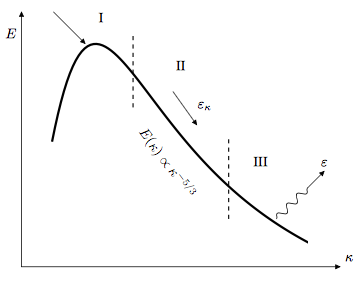
\includegraphics[width=0.5\textwidth]{figures/EnergySpectrum.png}
  \caption{Energy spectrum \cite{Lada}.}\label{fig:cascade}
\end{figure}

There exists a wide range of turbulence models that resolve different magnitude of turbulent scales. In Figure \ref{fig:modelling} the differences between modelling techniques, in terms of modelled and resolved turbulence, is shown in the form of energy, E, as a function of wavelength, $\kappa$. The simplest modelling techniques are the RANS family of models, where all turbulence is modelled by time averaging the governing equations. In RANS, a local time step is used, which means that the time-step is different for every cell, calculated as a function of the flow velocity, speed of sound and CFL number. Using local time-steps is used for faster convergence. The Unsteady RANS (URANS) family of models on the other hand, use a global time-step. This means that the very largest temporal scales can be resolved. For both RANS and URANS, a large time-step can be used as the grid can be relatively coarse to achieve grid independency. The LES equations are obtained by applying a spatial filtering to the governing equations instead of the time averaging method used in the RANS models. This results in the smaller scales being modelled whereas the larger ones are resolved. The definition of small and large is determined by the grid, where the small scales are too small to be resolved by the grid. The small eddies are therefore usually referred to as the sub-grid-scales (SGS) and the limit of the modelled scales is referred to as the cut-off limit (see $\kappa _\text{cut-off}$ in Figure \ref{fig:modelling}). The larger scales are resolvable by the grid where the lower limit is usually of a similar order of magnitude as few cells. According to Spalart \cite{YoungsPersonGuide}, eddies with wavelengths of about five cells are resolved, they are however not very accurate as they lack the connection to the smaller scales. Instead they are dominated by the modelled viscosity from the SGS model. An example of the large and small scales is shown in Figure \ref{fig:Scales} where the dashed-line curve represents an SGS whereas the whole-line one represents what could be the lower limit for the larger scales. The time-step for LES should be relatively small compared to URANS as it is determined by the smallest resolved scales on a significantly finer grid. 
\begin{figure}[h]
   \centering
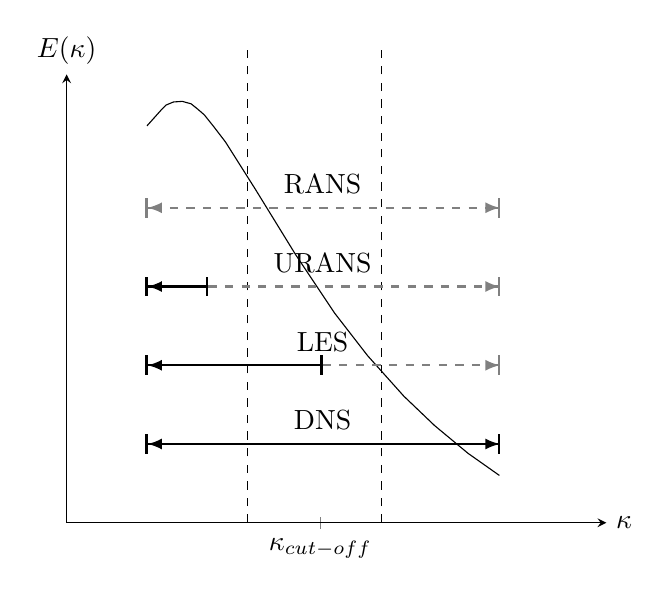
\begin{tikzpicture}
    \begin{axis}[
                %grid=both,
                ymin=0,
                ymax=1,
                xmax=1,
                xmin=0,
                xtick = 0.47,
                xticklabel=$\kappa _{\text{cut-off}}$,
                ytick = \empty,
                yticklabel=\empty,
                %minor tick num=1,
                axis lines = middle,
                xlabel=$\kappa$,
                ylabel=$E(\kappa)$,
                xlabel style={at=(current axis.right of origin), anchor=west},
                ylabel style={at=(current axis.above origin), anchor=south},
                %label style = {at={(ticklabel cs:1.1)}}
                ]
\end{axis}

\coordinate (B) at (6*0.17,                6*0.84);
\coordinate (F) at (6*0.200207468879668,   6*0.8737659643261302);
\coordinate (G) at (6*0.2105809128630705,  6*0.8841421027105674);
\coordinate (H) at (6*0.22614107883817425, 6*0.890615401196314);
\coordinate (I) at (6*0.24481327800829872, 6*0.8918898528857034);
\coordinate (J) at (6*0.2634854771784232,  6*0.8866707980815864);
\coordinate (K) at (6*0.2780082987551867,  6*0.8749636255860322);
\coordinate (L) at (6*0.2914937759336099,  6*0.8632578002909952);
\coordinate (M) at (6*0.3112033195020747,  6*0.8385568788058414);
\coordinate (N) at (6*0.3360995850622406,  6*0.8060570135258931);
\coordinate (P) at (6*0.39937759336099576, 6*0.7059748342943364);
\coordinate (Q) at (6*0.48340248962655596, 6*0.5695020746887967);
\coordinate (R) at (6*0.567427385892116,   6*0.4434189254728673);
\coordinate (S) at (6*0.6369294605809128,  6*0.3537182734278170);
\coordinate (T) at (6*0.7136929460580912,  6*0.2679042948752492);
\coordinate (U) at (6*0.7790456431535268,  6*0.2054817589049954);
\coordinate (V) at (6*0.8495850622406638,  6*0.1469485908282588);
\coordinate (W) at (6*0.9159751037344398,  6*0.1001091232419033);

%  \draw [gray!50]  (A) -- (B);
  \draw [] plot [smooth, tension=0.] coordinates {(B) (F) (G) (H) (I) (J) (K) (L) (M) (N) (P) (Q) (R) (S) (T) (U) (V) (W)};

  \draw [dashed] (2.3,0.) -- (2.3,6);
  \draw [dashed] (4.,0.) -- (4.,6);

  \draw [|latex-,thick] (1.,1.) -- (1.1,1);
  \draw [-|,thick] (5.4,1.) -- (5.5,1);
  \node at (3.25,1) [yshift=0.3cm] {DNS};
  \draw [-latex, thick] (1.,1.) -- (5.5,1);

  \draw [|latex-|,thick] (1.,2.) -- (3.25,2);
  \draw [-|,dashed, gray, thick] (5.4,2.) -- (5.5,2);
  \node at (3.25,2) [yshift=0.3cm] {LES};
  \draw [-latex,dashed, gray, thick] (3.25,2.) -- (5.5,2);

  \draw [|latex-|,thick] (1.,3.) -- (1.8,3);
  \draw [-|,dashed, gray, thick] (5.4,3.) -- (5.5,3);
  \node at (3.25,3) [yshift=0.3cm] {URANS};
  \draw [-latex,dashed, gray, thick] (1.8,3.) -- (5.5,3);

  \draw [|latex-,thick, gray, dashed] (1.,4.) -- (1.1,4);
  \draw [-|,dashed, gray, thick] (5.4,4.) -- (5.5,4);
  \node at (3.25,4) [yshift=0.3cm] {RANS};
  \draw [-latex,dashed, gray, thick] (1.1,4.) -- (5.5,4);

\end{tikzpicture}


   \caption{Energy spectrum with clarifications to what extent the different modelling procedures resolve (--) and model ({\color{gray}- -}) the turbulence.}
  \label{fig:modelling}
\end{figure}

In Direct Numerical Simulations (DNS) the whole turbulence spectrum is resolved. This is however very expensive and is not a practical option for high Reynolds number flows with complicated geometries as the spatial and temporal resolutions are determined by the Kolmogorove length and time scales (the smallest scales from section III in Figure \ref{fig:cascade}), respectively, which results in a very fine grid and very small time-step. 
\begin{figure}[h]
  \centering

\begin{tikzpicture}
  \coordinate (A) at (0,0);
  \coordinate (B) at (2,2);
  %Arrows
%  \draw[-latex] (A)--(B);
  %circles - First
  \circledarrow{thick,very thick, dashed}{3,3}{0.5cm};
  \circledarrow{thick,very thick}{3,3}{2.5cm};
  \draw[step=1.0cm,gray,thick] (0,0) grid (6,6);
\end{tikzpicture}
  \caption{Modelled (- -) and resolved (--) scales.}\label{fig:Scales}
\end{figure}

%\begin{figure}[H]
%  \centering
%  \includegraphics[width=0.5\textwidth]{../figures/Energy}
%  \caption{Modelling fraction of different turbulence models}\label{fig:modelling}
%\end{figure}




%
%   .--~*teu.
%  dF     988Nx
% d888b   `8888>
% ?8888>  98888F
%  "**"  x88888~
%       d8888*`
%     z8**"`   :
%   :?.....  ..F
%  <""888888888~
%  8:  "888888*
%  ""    "**"`
%
% http://patorjk.com/software/taag/#p=display&f=Fraktur  --  Text to ASCII graphics
%
%%%%%%%%%%%%%%%%%%%%%%%%%%%%%%%%%%%%
%%%%%%%%%%%%%%%%%%%%%%%%%%%%%%%%%%%%
\chapter{Methodology\label{ch:NM}}
The finite volume in-house CFD solver for compressible flows, called G3D::Flow, is used. It is based on a family of codes developed by Eriksson \cite{g3dflow}. The solver is developed and maintained at the Division of Fluid Dynamics at Chalmers University of Technology. It uses three-stage Runge-Kutta time marching method with a third-order accurate upwind-biased scheme for all convective terms and a second-order accurate compact centered scheme for all diffusive terms. For more details on the numerical scheme see Eriksson \cite{g3dflow} or Andersson et al. \cite{g3dflowNA}.

The Spalart-Allmaras one-equation turbulence model (SA) and the SA-based DDES model were implemented into the G3D::Flow solver. The implementation of the SA model is verified in Chapter \ref{ch:verification}, where the results are compared to well-established data. 
\section{Governing equations}
The governing equations on compressible, unsteady and viscid form are presented in Eq. \ref{eq:NS}. They are often referred to as the Navier-Stokes equations and consists of the continuity, momentum and energy equations, respectively.
\begin{equation} 
  \label{eq:NS}
  \begin{gathered}
    \frac{\partial {\rho}}{\partial t} + \frac{\partial \left({\rho} {u}_j \right)}{\partial x_j} = 0 \\
    \frac{\partial \left( {\rho} {u}_i \right)}{\partial t} + \frac{\partial\left({\rho} {u}_i {u}_j \right)}{\partial x_j} = -\frac{\partial p}{\partial x_i} + \frac{\partial {\sigma} _{ij}}{\partial x_j} \\
    \frac{\partial \left( {\rho} {e}_0\right)}{\partial t} + \frac{\partial \left({\rho} {e}_0 {u}_j\right)}{\partial x_j}= -\frac{\partial {p}{u}_j}{\partial x_j}+\frac{\partial}{\partial x_j}\left(C_p\frac{\mu}{Pr}\frac{\partial {T}}{\partial x_j}\right)+\frac{\partial}{\partial x_j}\left({u}_i\sigma_{ij}\right)
  \end{gathered}
\end{equation}
where ${\sigma} _{ij}$ is the viscous stress tensor
\begin{equation}
  {\sigma} _{ij} = \mu \left(2{S}_{ij}-\frac{2}{3}{S}_{mm}\delta _{ij}\right),
\end{equation}
${S}_{ij}$ is the strain rate tensor
\begin{equation}
  {S}_{ij}=\frac{1}{2}\left(\frac{\partial {u}_i}{\partial x_j}+\frac{\partial {u}_j}{\partial x_i}\right)
\end{equation}
and $Pr$ is the Prandtl number
\begin{equation}
  Pr = \frac{\mu C_p}{k}
\end{equation}
$C_p$ is the specific heat, $\mu$ the viscosity and k the thermal conductivity. The gas is assumed to be calorically perfect as the temperature in all simulations does not reach higher values than room temperature. The gas obeys the gas law and internal energy and enthalpy are linear functions of temperature
\begin{equation}
  \begin{aligned}
    e &= C_vT \\
    h &= C_pT \\
    C_v &= C_p-R
\end{aligned}
\end{equation}
To be able to solve this set of equations, all scales need to be resolved (DNS), that is, all scales down to the smallest Kolmogorov scales. However, like discussed in the previous chapter, this puts impossible requirements on the spatial and temporal resolution. Therefore, due to limitations in computational power, this is not and will not be possible for practical applications in the near future. This means that modelling techniques are needed to close the set of equations. 

%The $\tau _{ij}$ is the turbulent stress term which models the momentum transport due to turbulence. It is this term that is solved dependent on which turbulence model is used, where resolving it results in high demands on the mesh- and time-scale of the simulation, hence DNS. This term is then modelled to some extent when using less computationally demanding turbulence models.\\
%\begin{equation}
%  \tau _{ij} = \mu _t 2{S}_{ij}
%\end{equation}

\section{URANS}
%Favre averaging
Ensemble-averaging the governing equations has proven to be quite successful. For an arbitrary variable $\phi$ the averaging is expressed as
\begin{equation}
  \overline{\phi} = \lim\limits_{N \to \infty}\frac{1}{N}\sum ^{N} _{i=1} \phi_i,  \quad \phi = \overline{\phi}+\phi'
\end{equation}
where $\phi'$ denotes the fluctuating part of $\phi$. However, by ensemble-averaging the compressible form of the Navier-Stokes equations additional unknown terms, compared to the incompressible form, have to be modelled. To avoid those extra terms, a density weighted average procedure (also called Favre-averaging \cite{Favre1969}) is often used on top of the ensemble-averaging. The Favre-averaging of a flow variable ${\phi}$ is defined as 
\begin{equation}
  \hat{\phi} = \frac{\overline{\rho \phi}}{\bar{\rho}}
\end{equation}
and the decomposition of instantaneous flow properties reads
\begin{equation}
  \phi = \hat{\phi}+\phi'' = \frac{\overline{\rho \phi}}{\bar{\rho}}+\phi''
\end{equation}
where the $\phi''$ term represents the combination of the Reynolds decomposition fluctuating component $\phi'$ and the density fluctuations. The term $\bar{\phi}$ is the mean component of a specific variable. $\hat{\phi}$ can be thought of as the low frequency component whereas $\phi''$ represents high frequency one.
Applying the Favre-averaging method in a combination to the ensamble-averaging on the governing equations
\begin{equation} 
  \label{eq:NSFavre}
  \begin{gathered}
    \frac{\partial \overline{\rho}}{\partial t} + \frac{\partial \left(\overline{\rho} \hat{u}_j \right)}{\partial x_j} = 0 \\
    \frac{\partial \left( \overline{\rho} \hat{u}_i \right)}{\partial t} + \frac{\partial\left(\overline{\rho} \hat{u}_i \hat{u}_j \right)}{\partial x_j} = -\frac{\partial \overline{p}\delta _{ij}}{\partial x_i} + \frac{\partial \hat{\sigma} _{ij}}{\partial x_i}+\frac{\partial \tau _{ij}}{\partial x_j} \\
    \frac{\partial \left( \overline{\rho} \hat{e}_0\right)}{\partial t} + \frac{\partial \left(\overline{\rho} \hat{e}_0 \hat{u}_j\right)}{\partial x_j}= -\frac{\partial \overline{p}\hat{u}_j}{\partial x_j}+\frac{\partial}{\partial x_j}\left(C_p\frac{\mu}{Pr}\frac{\partial {T}}{\partial x_j}+q_j^t\right)+\frac{\partial}{\partial x_j}\left(\hat{u}_i\left(\overline{\sigma} _{ij} + \tau_{ij}\right)\right)\\
    -\frac{1}{2}\frac{\partial}{\partial x_j}\overline{\rho}\left(\widehat{u_iu_iu}_j-\widehat{u_iu}_i\hat{u}_j\right)
  \end{gathered}
\end{equation}
where $\hat{\sigma} _{ij}$ is the Favre-averaged viscous stress tensor
\begin{equation}
  \hat{\sigma} _{ij} = \mu \left(2\hat{S}_{ij}-\frac{2}{3}\hat{S}_{mm}\delta _{ij}\right),
\end{equation}
and $\hat{S}_{ij}$ is the Favre-averaged strain rate tensor
\begin{equation}
  \hat{S}_{ij}=\frac{1}{2}\left(\frac{\partial \hat{u}_i}{\partial x_j}+\frac{\partial \hat{u}_j}{\partial x_i}\right)
\end{equation}
If the Favre-averaged equations (Eqns. \ref{eq:NSFavre}) are compared to the Navier-Stokes equations (Eqns. \ref{eq:NS}), the Favre-averaged equations resemble the original ones but the Favre-averaged quantities are solved with extra stress terms. The triple velocity correlation term in the energy equation is usually neglected which leaves out two additional terms, the turbulent stresses and heat flux. The turbulent stress term 
\begin{equation}
  \begin{aligned}
    \tau _{ij}  &= -\overline{\rho}\left(\widehat{u_iu}_j-\hat{u}_i\hat{u}_j\right)\\
                &= -\overline{\rho}\left(\underbrace{\left(\widehat{\hat{u}_i\hat{u}}_j-\hat{u}_i\hat{u}_j\right)}_I+\underbrace{\left(\widehat{u_i''\hat{u}}_j+\widehat{\hat{u}_iu''}_j\right)}_{II}+\underbrace{\widehat{u''_iu''}_j}_{III}\right)
  \end{aligned}
\end{equation}
consist of three different terms, where term $I$ is called the Leonard stresses, $II$ the cross stresses and $III$ the Reynolds stresses, where the Leonard and cross stresses are usually neglected. 

The turbulent heat flux is given as
\begin{equation}
  q_j^t = -C_p\overline{\rho}\left(\widehat{Tu}_j-\hat{T}\hat{u}_j\right) \label{eq:FavreEnd}
\end{equation}
This means that the closed set of equations formed by the Navier-Stokes equations are not enclosed by the averaging technique, resulting in a need for modelling the unknown turbulent stress terms.

To be able to evaluate the turbulent stress term, i.e. to close the set of equations, turbulence models are introduced. There are many different models available but Spalart and Allmaras \cite{SA} derived a single equation turbulence model where it is assumed that the turbulent stress is given by the relation 
\begin{equation}
  \tau_{ij} = -2\nu_t{S}_{ij}
\end{equation}
where $\nu_t$ is the kinematic turbulent viscosity.

The SA model solves for a new turbulence variable, $\tilde{\nu}$. The model, on conservative and compressible form is presented in Eq. \ref{eq:SA}, excluding a trip term ($f_{t1}$) that was included in the original form of the equation \cite{SA,SAmod}.
\begin{equation}
\begin{aligned}
  &\frac{\partial\bar{\rho}\tilde{\nu}}{\partial t}+\frac{\partial}{\partial x_j}\left(\bar{\rho}{u}_i{u}_j\right) = \tilde{S}\tilde{\nu}\left(1-f_{t2}\right)c_{b1}\bar{\rho}+\frac{1}{\sigma}\frac{\partial}{\partial x_j}\left(\bar{\rho} \left(\nu+\tilde{\nu}\right)\frac{\partial \tilde{\nu}}{\partial x_j}\right)\\
  &+\frac{c_{b2}}{\sigma}\bar{\rho}\left(\frac{\partial \tilde{\nu}}{\partial x_j}\right)^2-\bar{\rho}\left(c_{w1}f_w-\frac{c_{b1}}{\kappa ^2}f_{t2}\right)\left(\frac{\tilde{\nu}}{d}\right)^2+\frac{1}{\sigma}\left(\nu+\tilde{\nu}\right)\frac{\partial \bar{\rho}}{\partial x_j}\frac{\partial \tilde{\nu}}{\partial x_j}\label{eq:SA}
\end{aligned}
\end{equation}
where  
\begin{equation}
  \begin{gathered}
    \nu_t = \tilde{\nu}f_{v1}, \qquad f_{v1}=\frac{\chi^3}{\chi^3+c_{v1}^3},\qquad \chi = \frac{\tilde{\nu}}{\nu}\\
  \tilde{S} = S + \frac{\tilde{\nu}}{\kappa ^2 d ^2}f_{v2}, \qquad f_{v2}=1-\frac{\chi}{1+\chi f_{v1}}\\
  f_w=g\left(\frac{1+c_{w3}^6}{g^6+c_{w3}^6}\right)^{1/6},\quad g=r+c_{w2}\left(r^6-r\right), \quad r=\frac{\tilde{\nu}}{\tilde{S}\kappa^2d^2}\\
    f_{t2} = c_{t3}exp\left(-c_{t4}\chi^2\right)\label{eq:SAf}
  \end{gathered}
  \end{equation}
and the corresponding constants 
\begin{equation}
  \begin{aligned}
    c_{b1}&=0.1355, & \sigma&=2/3, &  c_{b2}&=0.622,                                          &  \kappa&=0.41, \\
    c_{w2}&=0.3,    & c_{w3}&=2,   &  c_{v1}&=7.1,                                            &  c_{t3}&=1.2, \\
    c_{t3}&=0.5,    &       &      &  c_{w1}&=c_{b1}/\kappa^2+\left(1+c_{b2}\right)/\sigma.   &        &
  \end{aligned}
\end{equation}
In the SA model the turbulence stress term $\tau _{ij}$, also called the Reynolds stress term for RANS models, accounts for the effects of the entire energy spectrum off all length scales on the average flow field. This means that all turbulence is modelled. 

\section{LES}
Compared to the URANS governing equations, the LES equations are written in the same way, with the modification that instead of applying an ensemble-averaging technique, a spatial filtering is used. That means for a filtered arbitrary variable $\phi$
\begin{equation}
  \overline{\phi}(x,t) = \frac{1}{\Delta x}\int ^{x+0.5\Delta x} _{x-0.5\Delta x} \phi(\xi,t) d\xi, \quad \phi = \overline{\phi}+\phi'
\end{equation}
The procedure is the same as for the ensemble-averaging where the Favre-averaging approach is applied to the governing equations, gives a result similar to the RANS equations with the fundamental difference that $\left(\bar{\bullet}\right)$ stands for spatial filtering instead of ensemble-averaging. Furthermore, as the finite volume discretization is used, the local control volume based on the computational grid represents the spatial filtering (i.e. implicit filter). In practice, the difference between RANS and LES, in addition to the different filtering techniques, is to what extent the Reynolds stresses are modelled (much greater for RANS). The turbulent stresses are treated in a different way compared to RANS. The LES stresses that are not resolved are modelled using an SGS models, where the zero-equation Smagorinsky model \cite{Smagorinsky} is frequently used
\begin{equation}
  \begin{aligned}  \tau_{ij} - \frac{1}{3}\delta_{ij}\tau_{kk} &= -\nu_{sgs}\left(\frac{\partial \overline{u}_i}{\partial x_j}+\frac{\partial \overline{u}_j}{\partial x_i}\right) = -2\nu_{sgs}\overline{S}_{ij}\\
  \nu_{sgs} &=\left(C_S\Delta \right)^2\sqrt{2\overline{S}_{ij}\overline{S}_{ij}} \equiv \left(C_S\Delta \right)\left|\overline{S}\right|
  \end{aligned}
\end{equation}
and the filter-width is defined as the local grid size 
\begin{equation}
  \Delta = \left(\Delta V_{IJK}\right)^{1/3}
\end{equation}
As described in Chapter \ref{ch:Turbulence} the SGS are defined by the cut-off wavelength, where the length-scales lower than the cut-off are modelled whereas the larger ones are resolved. As a result, a finer mesh will result in a smaller portion of the energy spectrum being modelled. This means that a common mesh-dependency study can be difficult as the solution is mesh dependant and will approach DNS as the mesh is refined. Doing LES is computationally demanding as close to walls the larger scales are small, resulting in a need of fine mesh and consequently small time-steps. 

\section{DDES}
In previous sections the URANS and LES formulations were introduced. To be able to take the best out of each method, hybrid LES/RANS methods have been developed. The hybrid models simulate certain regions, usually attached or mildly separated boundary layers, using the URANS formulation of the governing equations, whereas the free-stream regions and largely separated areas are solved using LES. The transition between URANS and LES can be predefined (zonal methods) or calculated as a part of the model. This means that the boundary layer, were RANS-type models have proven to by quite reliable, can consist of relatively coarse mesh, lowering the computational cost substantially as fewer cells and a larger time-step can be used. Using the LES in the free-stream, means that transient flow features of the main flow are captured much better compared to the RANS-type models as a lower degree of modelling is applied.

Figure \ref{fig:FPDDES} shows a schematic view of a hypothetical inclined flat plate simulation using a hybrid modelling technique. In the figure the free-stream and the separated region on the suction side are simulated using LES whereas the attached boundary layer at the pressure side is simulated using RANS.
\begin{figure}[H]
  \centering
%\documentclass[12pt,english]{article}
%\usepackage{fullpage}
%\usepackage[T1]{fontenc} 
%\usepackage{helvet}
%\renewcommand{\familydefault}{\sfdefault}
%\usepackage{babel}
%\usepackage{amsmath}
%\numberwithick{equation}{section}
%\usepackage{hyperref}
%\usepackage{tikz,pgfplots}
%\usepackage{boldline} %To get thicker lines in tables
%\usepackage{float}    %For float on figures for exampel
%\usepackage{graphicx} %Figures
%
%\usepackage{sectsty}
%\allsectionsfont{\centering}
%
%\renewcommand{\thesubsection}{\Roman{subsection}} 
%\renewcommand{\thesubsubsection}{\Alph{subsubsection}} 
%
%\newcommand{\ignore}[1]{}
%\def\circledarrow#1#2#3{ % #1 Style, #2 Center, #3 Radius
%  \draw[#1,->] (#2) +(80:#3) arc(80:-260:#3);
%}
%
%\begin{document}
%
%\begin{figure}[H]
%  \centering
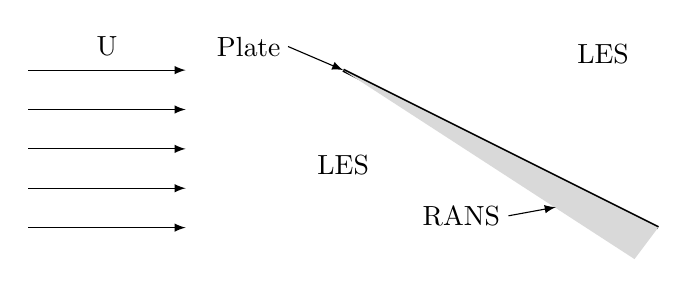
\begin{tikzpicture}
  \coordinate (A) at (0,0);
  \coordinate (B) at (2,0);
  \coordinate (C) at (0,0.5);
  \coordinate (D) at (2,0.5);
  \coordinate (E) at (0,1);
  \coordinate (F) at (2,1);
  \coordinate (G) at (0,1.5);
  \coordinate (H) at (2,1.5);
  \coordinate (I) at (0,2);
  \coordinate (J) at (2,2);
  %Arrows
  \draw[-latex] (A)--(B);
  \draw[-latex] (C)--(D);
  \draw[-latex] (E)--(F);
  \draw[-latex] (G)--(H);
  \draw[-latex] (I)--(J);
  %Plates
  \coordinate (AA) at (4,2);
  \coordinate (BB) at (8,0);
  \coordinate (CC) at (7.7,-0.4);
  \draw[very thick] (AA)--(BB);
  \fill[gray!30] (AA) -- (BB) -- (CC) -- cycle;
  %circles - First
  \circledarrow{thick, gray}{4.3,2}{0.1cm};
  \circledarrow{thick, gray}{4.65,1.95}{0.1cm};
  \circledarrow{thick, gray}{4.95,1.7}{0.1cm};
  \circledarrow{thick, gray}{5.4,1.5}{0.1cm};
  \circledarrow{thick, gray}{5.9,1.3}{0.1cm};
  \circledarrow{thick, gray}{6.3,1.1}{0.1cm};
  \circledarrow{thick, gray}{6.7,0.95}{0.1cm};
  \circledarrow{thick, gray}{7.1,0.7}{0.1cm};
  \circledarrow{thick, gray}{7.5,0.5}{0.1cm};
  \circledarrow{thick, gray}{8.0,0.3}{0.1cm};
  %Circles - second
  \circledarrow{thick, gray}{5.2,1.85}{0.15cm};
  \circledarrow{thick, gray}{5.7,1.7}{0.15cm};
  \circledarrow{thick, gray}{6.2,1.5}{0.15cm};
  \circledarrow{thick, gray}{6.6,1.3}{0.15cm};
  \circledarrow{thick, gray}{6.9,1.8}{0.15cm};
  \circledarrow{thick, gray}{7.2,1.0}{0.15cm};
  \circledarrow{thick, gray}{7.8,0.8}{0.15cm};
  \circledarrow{thick, gray}{8.2,0.95}{0.15cm};
  %Circle - third
  \circledarrow{thick, gray}{6.4,1.9}{0.2cm};
  \circledarrow{thick, gray}{7.0,1.45}{0.2cm};
  \circledarrow{thick, gray}{7.5,1.6}{0.2cm};
  \circledarrow{thick, gray}{7.8,1.2}{0.2cm};
  \circledarrow{thick, gray}{8.3,1.5}{0.2cm};
  
  \node at (1,2.3) {U};
  \node at (4,0.8)  {LES};
  \node at (7.3,2.2)  {LES};
  \node at (5.5,0.15) {RANS};
  \node at (2.8,2.3)  {Plate};

  \draw [-latex] (3.3,2.3)--(4.0,2.0);
  \draw [-latex] (6.1,0.15)--(6.7,0.26);
  %\draw[step=0.1cm,gray,very thick] (4,0) grid (9,2);

\end{tikzpicture}
%  \caption{???}
%  \label{fig:zones}
%\end{figure}
%\end{document}

  \caption{Hypothetical hybrid simulation of an inclined flat plate.}\label{fig:FPDDES}
\end{figure}

The hybrid LES/RANS model DDES is based on the original Detached Eddy Simulation (DES) model \cite{DES97}. The hybrid model uses the SA one-equation turbulence model when simulating RANS regions whereas it is used as an SGS model in LES regions. To apply the SA model as an SGS model, a length scale is modified to account for the change from RANS to LES. The wall distance $d$, which is the SA-model length scale, is substituted in Eqns. \ref{eq:SA} and \ref{eq:SAf} for the modified length scale $\tilde{d}$, which is defined in Eq. \ref{eq:DDES} but this is the procedure for both DES and DDES. 

The DDES is an improvement from the original DES model as the switching between LES and RANS is not only governed by cell size but is also dependent on the flow itself. This has great benefits, as the risk of premature switching from RANS to LES for grids with stream-wise grid spacing of similar size as the boundary layer thickness, is quite high for the DES model. The premature switching is known to cause grid induces separation \cite{DDES}. This puts flows with strong gradients in the stream-wise direction in a specific danger. If the stream-wise grid size is of similar size as the boundary layer the original DES model extends the LES region into the boundary layer where the grid is not fine enough to be capable in resolving the turbulent stresses. To improve the boundary layer behaviour, a shielding function was added to the DES formulation, resulting in the DDES model. The shielding function protects the boundary layer from being solved using the LES formulation.
\begin{equation}
  f_d = 1-\tanh\left[(8r_d)^3\right].
  \label{eq:fd}
\end{equation}
$f_d$ is designed to be 0 in the boundary layer but 1 outside of it. The $r_d$ is similar to the $r$ function in the SA model
\begin{equation}
  r_d = \frac{\nu+\nu_t}{\sqrt{U_{i,j}U_{i,j}}\kappa^2 d^2}
  \label{eq:rd}
\end{equation}
The length scale, introduced in the original DES model, was only based on the wall distance and the grid spacing $\Delta$,
\begin{equation}
  \tilde{d}_{DES}=min(d,C_{DES}\Delta)
  \label{eq:DES97}
\end{equation}
but like discussed earlier this can result in a grid induced separation, which resulted in the adjustments made in the DDES version, where a modified length scale was introduced where a dependency on the boundary layer shielding function $f_d$ was included
\begin{equation}
  \tilde{d}_{DDES} = d-f_dmax(0,d-C_{DES}\Delta).
  \label{eq:DDES}
\end{equation}
When $f_d=0$, the model behaves like a RANS model while $f_d=1$ results in the original DES model shown in Eq.~(\ref{eq:DES97}). Outside the boundary layer the DES model should be in LES mode. Shur et al. \cite{DES99} compared the SA as a SGS model for the original DES model to the Smagorisnky SGS model and experimental data. There, a good agreement was achieved when simulating isotropic turbulence using the filtering factor $C_{DES}=0.65$.

The coefficients in the $f_d$ function where calibrated using a flat-plate boundary layer but recent studies have shown that some modifications might be needed for it to perform well for specific problems. Ashton \cite{Ashton2016} presented work for a three element airfoil, where a problem regarding the shielding function was encountered. The conclusion was that even though the DDES model was applied, the stream-wise and span-wise grid sizes were to fine. The fine mesh, in addition to strong pressure gradients over curved surfaces, caused the shielding function to break down and allow for LES mode inside the boundary layer. Probst et al. \cite{Probst2010} encountered a similar problem for a simple airfoil. In their opinion a coarser mesh was not an option as high resolution in the stream-wise direction was required to be able to capture the adverse pressure gradient over the wing. Instead, they suggested a slight modification to the $f_d$ function where the value of the coefficient in front of $r_d$ was increased from 8 to 16, shown in Eq. \ref{eq:fdmod}. 
\begin{equation}
  f_d^{mod} = 1-\tanh\left[(16r_d)^3\right].
  \label{eq:fdmod}
\end{equation}
This shows that even though the DDES model modification to handle ambiguous grids is implemented, the solution is still sensitive to stream-wise grid spacing. Both versions of the $f_d$ function were tested and evaluated for a single pree-swirler module, where better performance was obtain using the modified function but further analyses have to be made [Paper A].

Furthermore, it has been shown that when using the SA model as a base model for DDES, $f_{t2}$ should be excluded from the equations. It has the tendency to cause the boundary layer to stay laminar over the geometry on finer grids \cite{Vatsa2017}.



%   .x~~"*Weu.
%  d8Nu.  9888c
%  88888  98888
%  "***"  9888%
%       ..@8*"
%    ````"8Weu
%   ..    ?8888L
% :@88N   '8888N
% *8888~  '8888F
% '*8"`   9888%
%   `~===*%"`
%
%%%%%%%%%%%%%%%%%%%%%%%%%%%%%%%
%%%%%%%%%%%%%%%%%%%%%%%%%%%%%%%
\chapter{Unpublished results\label{ch:sim}}%Computaional model of the experimental rig\label{ch:sim}}
To study the flow of an ICD, an experimental test rig has been built at GKN Aerospace in Trollhättan (described in more details in Chapter \ref{ch:engine}). Performing simulations on a computational model representing the experimental test rig requires a high-quality grid and predefined boundary conditions. In the following sections the computational domain and setup are introduced followed by an unpublished comparison between the in-house solver G3D::Flow and the commercial solver CFX.
\section{Computational domain}
In Figure \ref{fig:rig} the computational domain is shown. It is a 3D-extension of the setup presented in Figure \ref{fig:schema} where the casing walls and the bleed pipe have been removed for visibility. As discussed in Chapter \ref{ch:Intro}, the domain is split into four main modules; PSW, bleed pipe, OGV and the ICD.
\begin{figure}[H]
  \centering
  \begin{tikzpicture}
    \node[anchor=south west,inner sep=0] at (0,0) {\includegraphics[width=9.05cm]{figures/RigBladesAndSurfaces.pdf}};
  \node at (3.3,5.4) {\bf{FT}};
  \draw[-latex] (3.0,5.4)--(2.65,5.0);
  \node at (4.05,5) {\bf{P$_\text{OGV}$}};
  \draw[-latex] (3.5,5)--(3.1,4.65);
  \node at (5.6,3.9) {\bf{P$_\text{DUCT}$}};
  \draw[-latex] (4.9,3.9)--(4.36,3.36);
  \node at (6.8,3.) {\bf{NRT}};
  \draw[-latex] (6.8,2.8)--(6.57,2.2);
  \node at (7.8,2.4) {\bf{FRT}};
  \draw[-latex] (7.8,2.2)--(7.54,1.8);
  \node at (3.6,1.1) {\bf{Strut}};
  \draw[-latex] (3.7,1.2)--(4,1.6);
    \node at (1.9,1.2) {\bf{OGV}};
  \draw[-latex] (1.9,1.4)--(2.2,1.8);
  \node at (0.3,3.8) {\bf{PSW}};
  \draw[-latex] (0.5,4.0)--(0.9,4.4);
    %\draw[help lines,step=.2] (0,0) grid (8.5,6);
\end{tikzpicture}
  \caption{3D representation of the computational setup.}\label{fig:rig}
\end{figure}

To be able to account for all interaction effects between different modules and blades, equal pitch for all domains is required. As one ICD module, which is the widest of the four modules, covers a 40$^{\circ}$ tangential sector, the rest has to match that sector width. To summarize, 5 PSW:s, 9 OGV:s and 1 strut are included in the CFD analysis. In Figures \ref{fig:meshPSW}-\ref{fig:meshDuct} the meshes for the PSW:s, OGV:s and strut's leading and trailing edges are shown. It is a multiblock, structured mesh with O-grids around the blades for a well resolved boundary layer.

\begin{figure}[h!]
  \centering
  \begin{minipage}{0.49\columnwidth}
  \includegraphics[width=6cm]{figures/PSWLeadingEdge.pdf}
  \end{minipage}
  \begin{minipage}{0.49\columnwidth}
  \includegraphics[width=6cm]{figures/PSWTrailingEdge.pdf}
  \end{minipage}
  \caption{PSW's leading and trailing edge meshes.} \label{fig:meshPSW}
\end{figure}
\begin{figure}[h!]
  \begin{minipage}{0.49\columnwidth}
  \includegraphics[width=6cm]{figures/OGVLE.pdf}
  \end{minipage}
  \begin{minipage}{0.49\columnwidth}
  \includegraphics[width=6cm]{figures/OGVTE.pdf}
  \end{minipage}
  \caption{OGV's leading and trailing edge meshes.} \label{fig:meshOGV}
\end{figure}
\begin{figure}[h!]
  \begin{minipage}{0.49\columnwidth}
  \includegraphics[width=6cm]{figures/DuctLE.pdf}
  \end{minipage}
  \begin{minipage}{0.49\columnwidth}
  \includegraphics[width=6cm]{figures/DuctTE.pdf}
  \end{minipage}  
  \caption{Strut's leading and trailing edge meshes.} \label{fig:meshDuct}
\end{figure}
The bleed pipe is axisymmetric and is therefore relatively simple to mesh. The 2D mesh, shown in Figure \ref{fig:bleed}, is rotated around the common ICD axis to obtain the 3D mesh. With this procedure, the bleed module is adjusted to match the tangential sectors of the surrounding modules. Upstream, the bleed pipe module is connected to the PSW:s and downstream to the OGV:s. The bleed pipe outlet is located at the upper surface of the module. The bleed pipe module is extended according to the findings in Paper B, where a shorter bleed pipe caused blocking and instabilities (see Paper B or Chapter \ref{ch:summary} for visualization of the old module). 

All meshes are generated using an in-house meshing tool, called G3dmesh. As the SA turbulence model is used and the risk of separation was estimated to be high, the boundary layers are resolved with $y^+<2$ for the first wall normal cells.

\begin{figure}[h!]
  \centering
    \begin{tikzpicture}
      \node[anchor=south west,inner sep=0] at (0,0) {    \includegraphics[width=9.05cm, height=6cm]{figures/BleedGrid2DBMFull.pdf}};
      \node[rotate=-90] at (9.1,1.8) {\bf{Bleed pipe outlet}};
      \node at (1.0,6.0) {\bf{PSW}};
      \node at (1.0,2.8) {\bf{OGV}};
    %\draw[help lines,step=.2] (0,0) grid (9,6);
    \end{tikzpicture}
\caption{2D representation of the bleed pipe mesh. Rotated $90^\circ$ clockwise.}\label{fig:bleed}
\end{figure}


\section{Computational setup}
The G3D::Flow simulations are performed using the SA turbulence model whereas the CFX simulations are performed using the k-$\omega$ SST turbulence model. This is done as the CFX solver only provides the SA model as a beta function.

A General Grid Interface (GGI) is used to calculate the fluxes traveling between the different modules, that is PSW:s, Bleed pipe, OGV:s and duct. The GGI ensures that all wakes and transient phenomena are transported interactively between the upstream and downstream modules. The boundary conditions applied are obtained from previous 1D calculations. At the inlet boundary, the total temperature and pressure are specified along with the velocity direction. The bleed pipe outlet is specified with a constant static pressure whereas at the duct's outlet is set as a mass-flow boundary. Predefining the mass-flow at the outlet forces the solution towards the correct through flow. The total temperature and the SA viscosity for the inlet boundary are the same for all bleed fractions, at a room temperature and $\tilde{\nu}_{in}=5\nu$. This value of $\tilde{\nu}$ represents a quite low turbulence intensity but as the main focus is on analysing the duct’s performance, it is assumed that the PSW generates sufficiently high turbulent flow, resulting in small effects from the inlet boundary. i.e. the flow downstream of the PSW is not affected by the low inlet turbulence value but without the PSW module in the upstream part of the configuration, there would probably be a need for specific treatment at the inlet boundary to ensure sufficient turbulence (for example higher $\tilde{\nu}$ value or synthetic turbulence). The pressure and mass-flow information cannot be presented due to confidentiality reasons.

Two operating conditions are simulated and compared between the two solvers. One lower-bleed fraction case, where $10\%$ of the inlet mass-flow is extracted through the bleed pipe and one high-bleed fraction case, where $40\%$ of the inlet mass-flow is extracted. Both cases have the same inlet boundary conditions whereas the bleed pipe outlet pressure and duct's outlet mass-flow are different.

%\begin{table}[H]
%  \caption{Boundary conditions} \label{tab:bc}
%  \centering
%\begin{tabular}{|c|c|c|c|c|c|}
%  \hline
%  \multicolumn{2}{|c|}{$\dot{m}_{bleed}=0.1$} & \multicolumn{2}{|c|}{$\dot{m}_{bleed}=0.4$} & \multicolumn{2}{|c|}{$\dot{m}_{bleed}=0.5$}\\
%  \hlineB{2}
%  $p_{in}$    & ?????   & $p_{in}$    & ????? & $p_{in}$    & ?????\\
%  \hline                                                           
%  $p_{t,in}$  & ?????   & $p_{t,in}$  & ????? & $p_{t,in}$  & ?????\\
%  \hline                                                           
%  $p_{out}$   & ?????   & $p_{out}$   & ????? & $p_{out}$   & ?????\\
%  \hline
%  $u_{in}$    & ?????   & $u_{in}$    & ????? & $u_{in}$    & ????? \\
%  \hline
%%  $T_{t,in}$          & 280     &               &      \\
%%  \hline
%%  $\tilde{\nu}_{in}$  & 5$\nu$  &               &      \\
%%  \hline
%\end{tabular}
%\end{table}

\section{Computational comparison}
In the following section the results from simulating the full experimental test rig using the G3D::Flow solver are compared to results obtained by using the commercial solver CFX. The following comparison along with the one done in Paper B are performed to give valuable feedback and increase the confidence in the in-house solver's performance.

The results are compared using radial profiles at the FT, NRT and FRT surfaces and the wall pressure at the intersection between the P$_\text{DUCT}$ and the hub and casing (for more details the reader is referred to Figure \ref{fig:rig}). Radial profiles of static pressure and total pressure are normalized with the corresponding maximum value. The total pressure is mass-flow averaged whereas the static pressure is area averaged. The radii are normalized with 
\begin{equation*}
  r_{norm} = \frac{r_{max}-r}{r_{max}-r_{min}}
\end{equation*}

Figure \ref{fig:FT10} shows the comparison for the $10\%$ bleed case at the FT surface. Radial profiles for the static and total pressure are presented. The two solvers agree very well. The static pressure profiles are almost identical, whereas insignificant difference is noticed near the hub for the total pressure.
\begin{figure}[h!]
  \centering
  \begin{minipage}{0.48\columnwidth}
  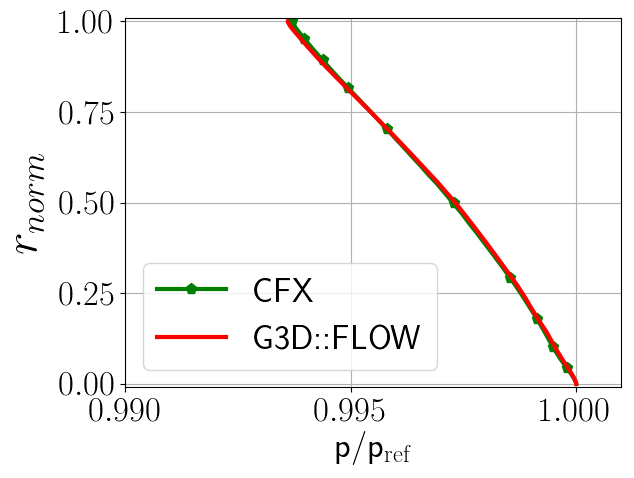
\includegraphics[width=1.\textwidth]{figures/PAaveB10_FT.png}
%    \caption*{Static pressure.}
  \end{minipage}
  \begin{minipage}{0.48\columnwidth}
  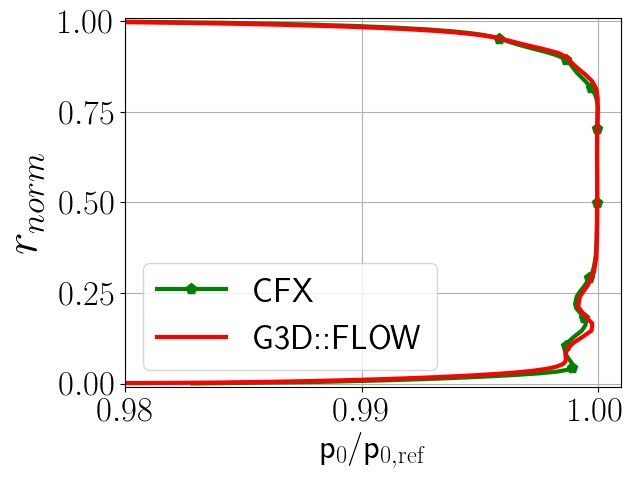
\includegraphics[width=1.\textwidth]{figures/P0MaveB10_FT.png}
%    \caption*{Total pressure.}
  \end{minipage}
  \caption{Radial profiles for $10\%$ bleed fraction case at the FT surface. Static pressure (left) and total pressure (right).} \label{fig:FT10}
\end{figure}

Moving further downstream, the discrepancies between the two solvers increases, as can be seen in Figure \ref{fig:NRT10}, where the profiles are evaluated at the NRT surface (see Figure \ref{fig:rig}). Major trends are similar for both solvers, where the region in the upper half of the duct differs in terms of the total pressure. The reason for the discrepancies might be caused by different prediction of the effects from the OGV wakes. The static pressure is identical for both solvers.

\begin{figure}[h!]
  \centering
  \begin{minipage}{0.48\columnwidth}
  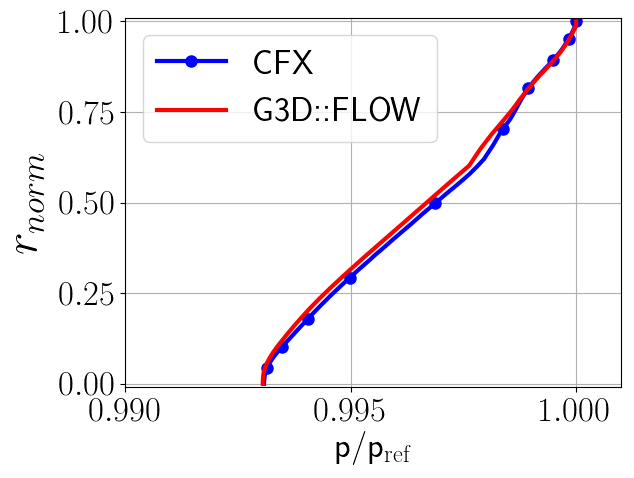
\includegraphics[width=1.\textwidth]{figures/PAaveB10_NRT.png}
%    \caption*{Static pressure.}
  \end{minipage}
  \begin{minipage}{0.48\columnwidth}
  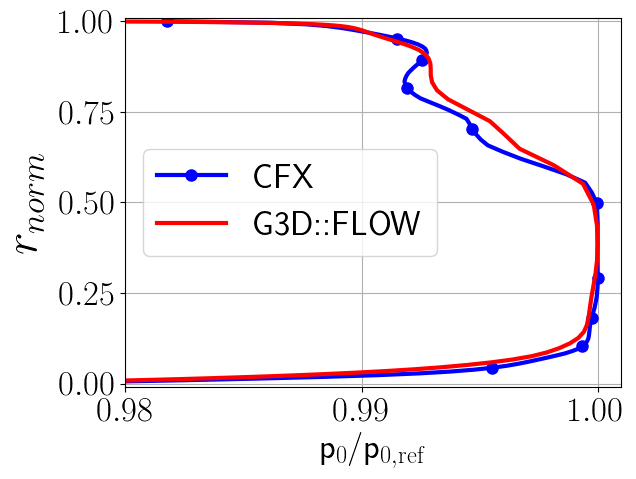
\includegraphics[width=1.\textwidth]{figures/P0MaveB10_NRT.png}
%    \caption*{Total pressure.}
  \end{minipage}
  \caption{Radial profiles for $10\%$ bleed fraction case at the NRT surface. Static pressure (left) and total pressure (right).} \label{fig:NRT10}
\end{figure}
Finally, Figure \ref{fig:FRT10} shows the comparison for the FRT surface (the most downstream evaluation plane - Figure \ref{fig:rig}). The figure shows that the two solvers, as for the NRT surface, differ in the upper half of the duct in terms of the total pressure. The static pressure is similar although larger differences are experienced compared to the other two surfaces, especially at the hub and casing.

Overall the two solvers compare well for the $10\%$ bleed fraction case, with some discrepancies in the upper half of the duct when considering the total pressure at the NRT and FRT surfaces. This behaviour might be explained by different predictions in the OGV wakes, but downstream of the strut the OGV wakes effects are mostly present in the upper half of the duct due to the S-shaped curvature, resulting in different local velocities and losses. The reason for this discrepancy in flow prediction could be explained by the fact that the SA model is used for G3D::Flow simulations whereas the k-$–omega$ SST model is used for CFX. At the trailing edge of the OGV blades, there is a minor separation areas but the two models are known to produce different results for separated flow.
\begin{figure}[h!]
  \centering
  \begin{minipage}{0.48\columnwidth}
  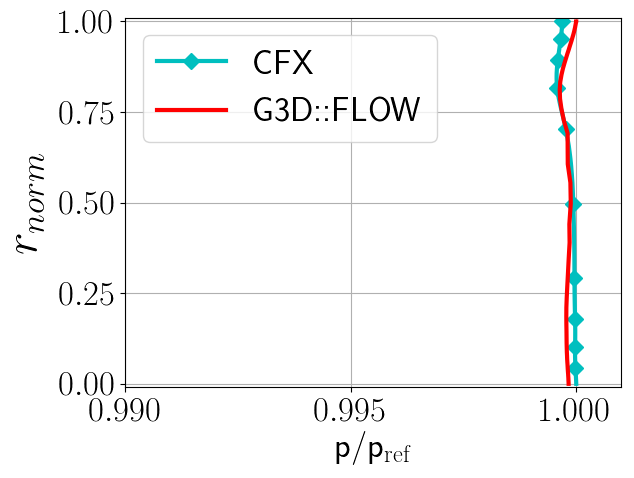
\includegraphics[width=1.\textwidth]{figures/PAaveB10_FRT.png}
%    \caption*{Static pressure.}
  \end{minipage}
  \begin{minipage}{0.48\columnwidth}
  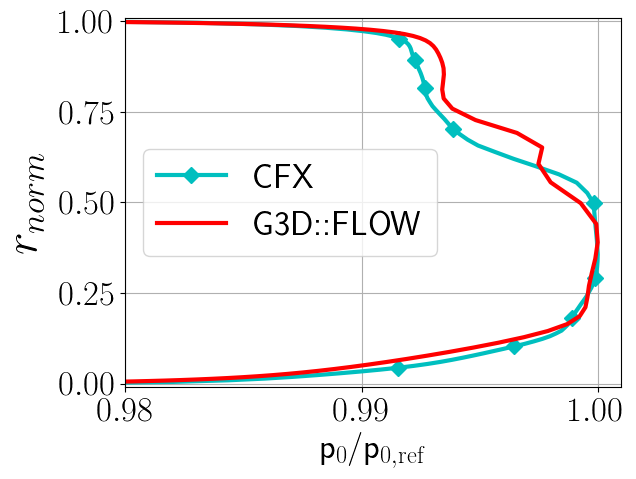
\includegraphics[width=1.\textwidth]{figures/P0MaveB10_FRT.png}
%    \caption*{Total pressure.}
  \end{minipage}
  \caption{Radial profiles for $10\%$ bleed fraction case at the FRT surface. Static pressure (left) and total pressure (right).} \label{fig:FRT10}
\end{figure}

In Figures \ref{fig:FT40}-\ref{fig:FRT40} the radial profiles are presented for the $40\%$ bleed fraction case at the same evaluation planes as for the $10\%$ case. At the FT surface, seen in Figure \ref{fig:FT40}, both solvers perform similarly for both bleed cases. This behaviour was expected since the main difference in the flow field is downstream of the bleed pipe. At the FT surface, small difference is noticed in the static pressure predictions comparing the two solvers, whereas they were identical for the $10\%$ bleed case. For the other two locations the difference is significant for all variables but some instabilities where encountered for the higher bleed case and therefore a completely converged solution was difficult to obtain. The general shape of the profiles generated by the two solvers is similar, with the largest difference found at the FRT casing for the total pressure.
\begin{figure}[h!]
  \centering
  \begin{minipage}{0.48\columnwidth}
  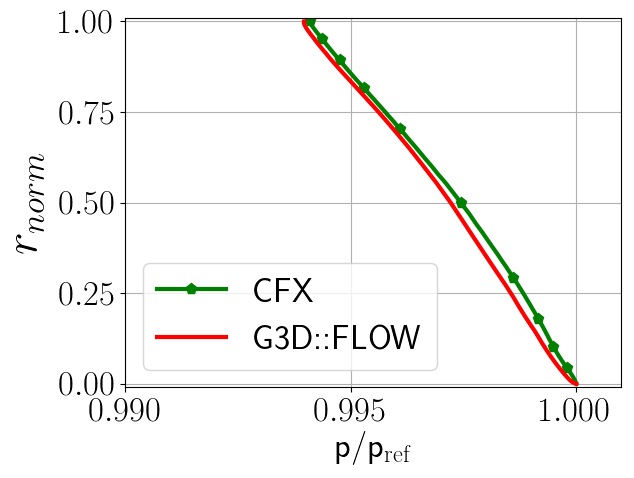
\includegraphics[width=1.\textwidth]{figures/PAaveB40_FT.png}
%    \caption*{Static pressure.}
  \end{minipage}
  \begin{minipage}{0.48\columnwidth}
  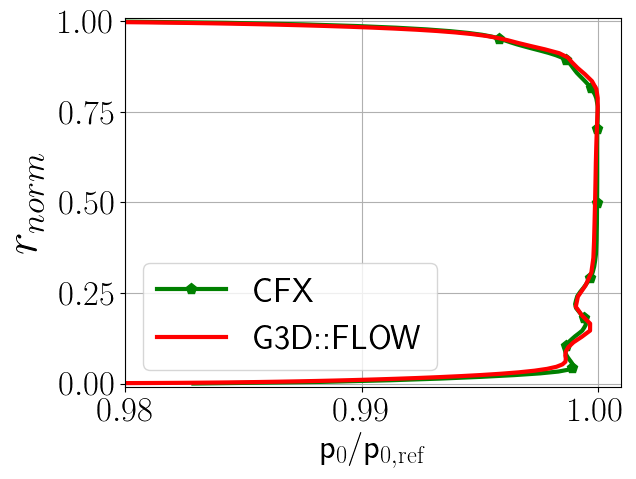
\includegraphics[width=1.\textwidth]{figures/P0MaveB40_FT.png}
%    \caption*{Total pressure.}
  \end{minipage}
  \caption{Radial profiles for $40\%$ bleed fraction case at the FT surface. Static pressure (left) and total pressure (right).} \label{fig:FT40}
\end{figure}

\begin{figure}[h!]
  \centering
  \begin{minipage}{0.48\columnwidth}
  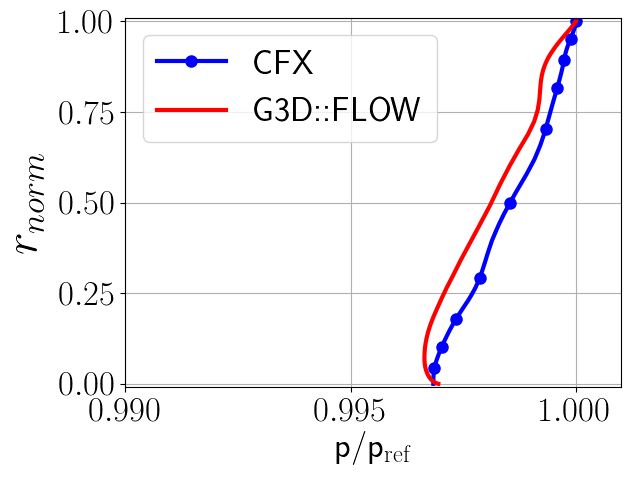
\includegraphics[width=1.\textwidth]{figures/PAaveB40_NRT.png}
%    \caption*{Static pressure.}
  \end{minipage}
  \begin{minipage}{0.48\columnwidth}
  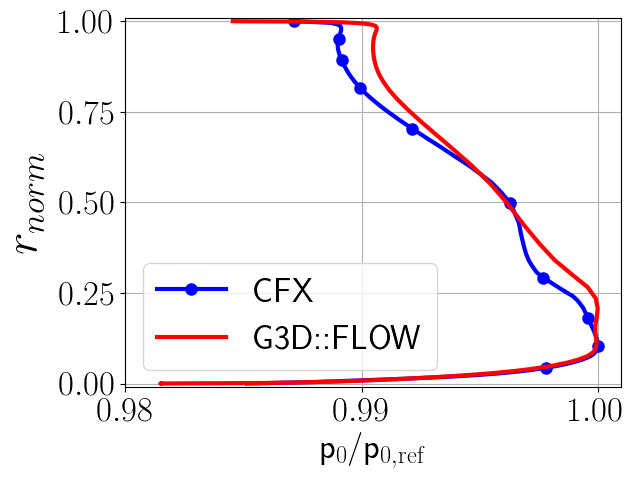
\includegraphics[width=1.\textwidth]{figures/P0MaveB40_NRT.png}
%    \caption*{Total pressure.}
  \end{minipage}
  \caption{Radial profiles for $40\%$ bleed fraction case at the NRT surface. Static pressure (left) and total pressure (right).} \label{fig:NRT40}
\end{figure}

\begin{figure}[h!]
  \centering
  \begin{minipage}{0.48\columnwidth}
  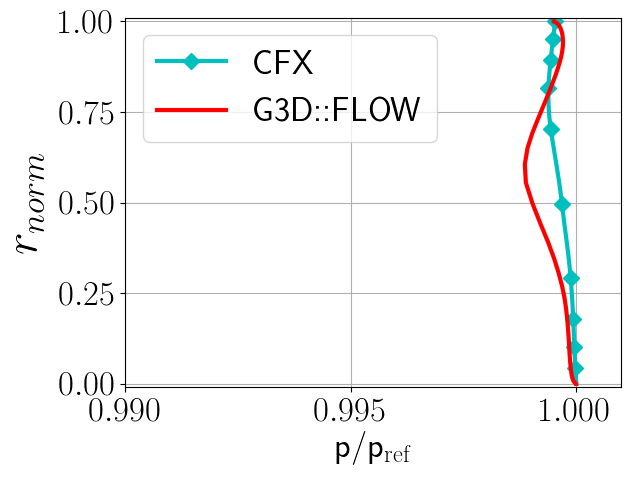
\includegraphics[width=1.\textwidth]{figures/PAaveB40_FRT.png}
%    \caption*{Static pressure.}
  \end{minipage}
  \begin{minipage}{0.48\columnwidth}
  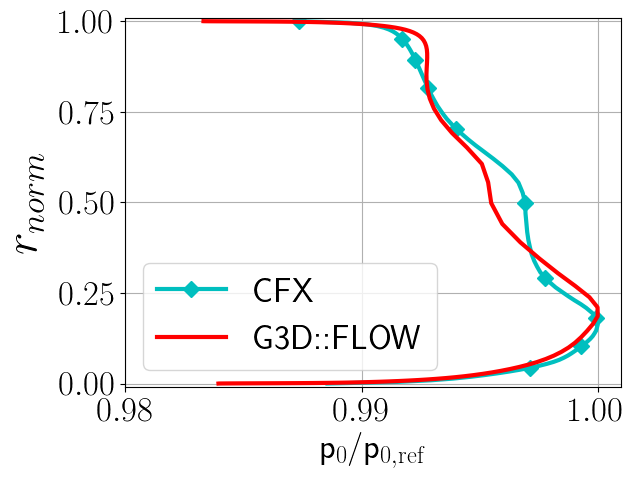
\includegraphics[width=1.\textwidth]{figures/P0MaveB40_FRT.png}
%    \caption*{Total pressure.}
  \end{minipage}
  \caption{Radial profiles for $40\%$ bleed fraction case at the FRT surface. Static pressure (left) and total pressure (right).} \label{fig:FRT40}
\end{figure}
In Figure \ref{fig:duct10} the normalized wall pressure at the intersection between the P$_\text{DUCT}$ and the end walls is compared between the two solvers for the $10\%$ bleed case. The total pressure at the inlet is used to normalize the pressure. The pressure is shown as a function of x-location, normalized with the distance from the leading edge of the strut to the duct's outlet. The vertical dashed lines represent the x-location of the leading and trailing edges of the strut. The pressure is in a good agreement between the two solvers for both hub and casing, with small deviation in the minimum value at the hub and small fluctuations at the casing. 
%
%The wall pressure in the S-shaped duct is not presented for the $40\%$ bleed case as strong pressure fluctuations at the walls made the comparison invalid. The reason for this was discussed in Paper B, and was related to the short bleed pipe effecting the flow with pressure fluctuations.
\begin{figure}[h!]
  \centering
  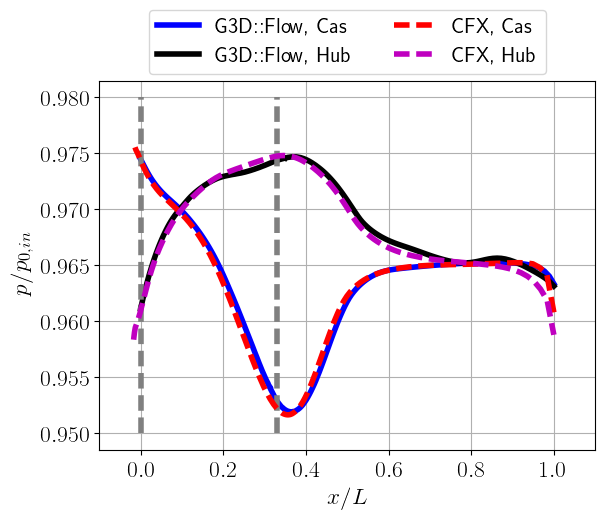
\includegraphics[width=.6\textwidth]{figures/CFXG3dDuct10.png}
    \caption{Normalized wall pressure in the ICD.} \label{fig:duct10}
\end{figure}

The normalized wall pressure for the $40\%$ bleed case is presented in Figure \ref{fig:duct40}, where the data is extracted at the same location as done for the $10\%$ bleed case. The two solvers differ significantly, where the pressure data seems to be offset through the ICD, with the G3D::Flow solver over predicting the pressure at the hub and under predicting it at the casing. As mentioned before, instabilities were initially encountered when simulating the higher bleed fraction resulting in a significant difference between CFD simulations and experimental data (Paper B). Furthermore, this case was more sensitive to an outlet mass-flow boundary conditions, resulting in divergence of the CFD solver. Due to this problem, the exact mass-flow compared to the CFX simulation, was not achieved as the outlet boundary was specified with a static pressure. The target mass-flow through the outlet boundary was $60\%$ of the inlet mass-flow but due to the difficulties in specifying the corresponding outlet pressure, the simulation resulted in outflow that was $57\%$ of the inflow. This discrepancy, between the outlet mass-flow calculated by the two solvers, might be enough to explain the difference in ICD wall pressures.
\begin{figure}[h!]
  \centering
  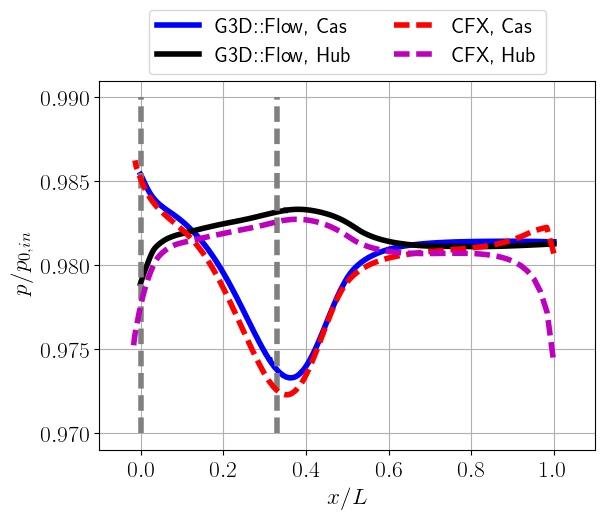
\includegraphics[width=.6\textwidth]{figures/CFXG3dDuct40.png}
    \caption{Normalized wall pressure in the ICD.} \label{fig:duct40}
\end{figure}

% 88        88
% 88        88
% 88        88
% 88        88
% 88        88
% 888888888888
%           88 
%           88 
%           88 
%           88
%           88  
%           
%%%%%%%%%%%%%%%%%%%%%%%%%%%%%%%
%%%%%%%%%%%%%%%%%%%%%%%%%%%%%%%
\chapter{SA turbulence model verification\label{ch:verification}}
To verify that the SA turbulence model is implemented correctly, a zero gradient boundary layer build up over a flat plate and a backward facing step (BFS) are simulated. 

A grid dependency study is performed and a comparison to results from the CFD solver CF3D, obtained from the NASA Turbulence Model Resources \cite{NASA}. As the SA model is a low Reynolds number model a $y^+$ value of about 1.0 is targeted as well as having a minimum of 10 cells inside the boundary layer to make sure that the boundary layer is well resolved. This is satisfied for most of the grids. 

The drag coefficient, $C_D$, is used for analysing the grid dependency for the flat plate boundary layer build up case
\begin{equation}
C_D=\frac{2F_D}{\rho_{ref}U^2_{ref}A}
\label{eq:CD}
\end{equation}
where $F_D$ is the drag force, $\rho_{ref}$ is a reference density, $U_{ref}$ is a reference velocity and $A$ is the surface in contact with the fluid.

Furthermore, the skin friction coefficient, $C_f$, is used for the grid dependency study as well as to compare the two solvers for both cases. The skin friction coefficient is defined as
\begin{equation}
  C_f = \frac{2\tau _w}{\rho_{ref}U^2_{ref}}
  \label{eq:CF}
\end{equation}
where $\tau _w$ is the wall shear stress
\begin{equation*}
  \tau_w = \mu \left( \frac{\partial u}{\partial y}\right)_{y=0}
\end{equation*}
$\mu$ is the dynamic viscosity, u is the flow parallel to the wall and y is the distance to the wall.

Additionally, the pressure coefficient is used to compare the two solvers when simulating the BFS, where
\begin{equation}
  C_p = \frac{2(p-p_{ref})}{\rho_{ref}U^2_{ref}}
  \label{eq:CP}
\end{equation}
where $p_{ref}$ is a reference pressure. 
\section{Flat plate simulation}
The computational setup for the 2D flat plate boundary layer build up can be seen in Figure \ref{fig:FP}. In the figure, the definition for the geometry and different boundaries are presented. The symmetry boundary, that is located before the wall, makes sure the inlet boundary will not be affected by the viscous wall.
\begin{figure}[h!]
  \centering
\begin{tikzpicture}
\begin{axis}[
  axis x line=bottom,
  axis y line=left,
%  scale only axis,
  xtick={-0.4,-0.2,...,2.1},
  ytick={-0.1,0,0.2,...,1.,1.1},
  xlabel={$\bf{x}$},
  ylabel={$\bf{y}$},
  xlabel style={below right},
  ylabel style={above left,rotate= -90},
  x=5cm,
  xmin=-0.4,
  xmax=2.1,
  ymin=-0.1,
  ymax=1.1]
\draw (5,10)--(240,10)--(240,110)--(5,110)--(5,10);
\draw[latex-latex,very thick] (5,13)--(40,13);
\node at (30,30) {symmetry};
  \draw[-latex,very thick] (30,27)--(30,13);
\draw[latex-latex,very thick] (40,13)--(240,13);
\node at (140,32) {visocus wall};
  \draw[-latex,very thick] (140,27)--(140,13);
\draw (40,10)--(40,17);
\node at (30,60) {inlet};
  \draw[latex-, very thick] (5,60)--(20,60);
\node at (210,60) {outlet};
  \draw[latex-, very thick] (240,60)--(222,60);
\node at (120,92) {symmetry};
  \draw[-latex, very thick] (120,98)--(120,110);
\end{axis}
\end{tikzpicture}
  \caption{Computational domain for the flat plate.}
  \label{fig:FP}
\end{figure}
In Table \ref{tab:FPBC} the boundary conditions for the simulations are given. The static pressure and temperature are defined relative to the ambient pressure and temperature. The reference values are $p_{ref}=1atm$ and $T_{ref}=294K$, i.e. the outlet pressure is the same as the ambient pressure. At the inlet the velocity direction and free-stream SA viscosity values are also given.
\begin{table}[H]
  \caption{Boundary conditions.} \label{tab:FPBC}
  \vspace{2mm}
  \centering
\begin{tabular}{|c|l|c|c|}
  \hline
    & $p_{\ast}/p_{ref}$ & $T_{\ast}/T_{ref}$ & $ \tilde{\nu}$  \\
  \hlineB{2}
  Inlet   & $1.02828$ & $1.008$ & $3\nu$ \\
  \hline
  Outlet  & $1.0$     & -       & - \\
  \hline
\end{tabular}
\end{table}
\subsection{Grid}
Five grids with different cell count are used for the grid dependency study. The information for each grid can be seen in Table \ref{tab:FPgrid} where Grid1 is the coarsest one and Grid5 the finest. $n_x$ is the number of nodes in x direction, $n_y$ the number of nodes in the y direction and $n_{tot}$ is the total number of nodes for each grid. The last column shows the average $y^+$ value for the first wall normal cells, averaged over the whole plate. The SA model is a low-Reynolds number model and therefore it is important to ensure that $y^+$ is smaller or equal to 1.0. This is satisfied for all grids except for the two coarsest grids, where the averaged $y^+$ value only slightly higher than one.
\begin{table}[H]
  \caption{Grid information for the flat-plate.} \label{tab:FPgrid}
  \vspace{2mm}
  \centering
\begin{tabular}{|c|r|r|r|c|}
  \hline
  Grid  & $n_x$ & $n_y$ & $n_{tot}$  & $y^+$  \\
  \hlineB{2}
  Grid1   & 35 & 25 & 875   & 1.25 \\
  \hline
  Grid2   & 69 & 49 & 3381  & 1.08 \\
  \hline
  Grid3   & 137& 97 & 13289 & 1.03 \\
  \hline
  Grid4   & 273& 193& 52689 & 1.00 \\
  \hline
  Grid5   & 545& 385& 209825& 0.97 \\
  \hline
\end{tabular}
\end{table}
Figure \ref{fig:FPgrid} shows Grid2. The cells grow exponentially from the leading edge of the plate towards the inlet and outlet as well as from the lower side of the domain towards the upper one. Furthermore, the leading edge of the plate is located at $x=0$.
\begin{figure}[H]
  \centering
\begin{tikzpicture}
  \node[anchor=south west,inner sep=0] at (0,0) {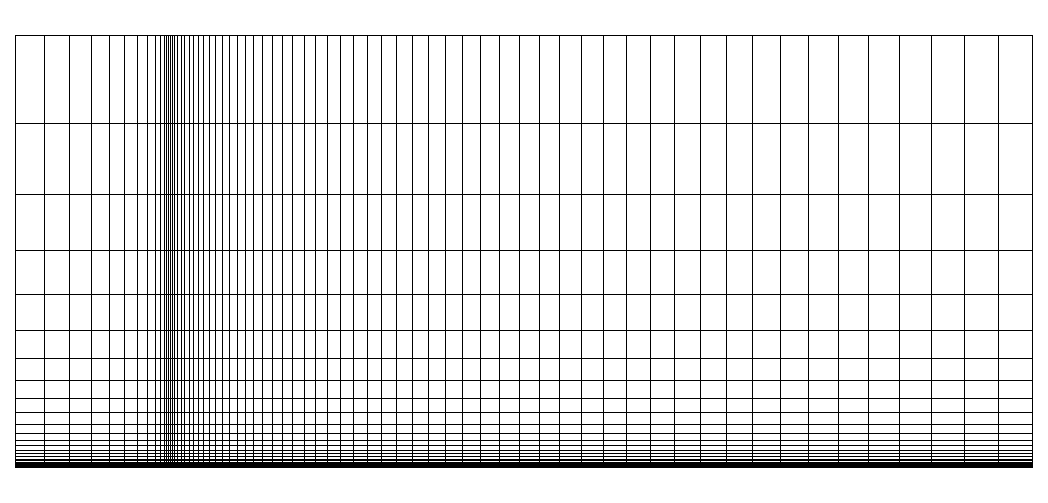
\includegraphics[width=0.8\textwidth]{figures/FP6949.png}};
  \draw[latex-] (1.75,0.37)--(1.9,0.12);
  \node at (3.7,0.12) {\scriptsize{Plate leading edge at $x=0$}};
  % \draw[help lines,step=.1] (0,0) grid (13,6);
\end{tikzpicture}
  \caption{Grid2, 69x49 cells.} \label{fig:FPgrid}
\end{figure}
\subsection{Results}
A grid dependency study was performed to ensure that the solution is independent off the grid. The drag and skin friction coefficients, Eq. \ref{eq:CD} and Eq. \ref{eq:CF} respectively, are compared for the different grids. The drag coefficient is estimated from the drag force calculated from the entire plate whereas the skin friction coefficient is evaluated at $x=0.97$. The comparison is presented in Figure \ref{fig:FPconstudy} where the convergence is clear for the local skin friction coefficient, Figure \ref{fig:FPconstudy} b). The drag coefficient is however not as clearly converged as can be seen in Figure \ref{fig:FPconstudy} a). The reason for this behaviour is probably that the skin friction, which is the only contributor to the drag in this case, is singular at the leading edge. This means that with finer grid, the values will increase infinitely. This result in a never-ending change for the integrated drag coefficient.
\begin{figure}[H]
  \centering
  \begin{minipage}{0.45\columnwidth}
  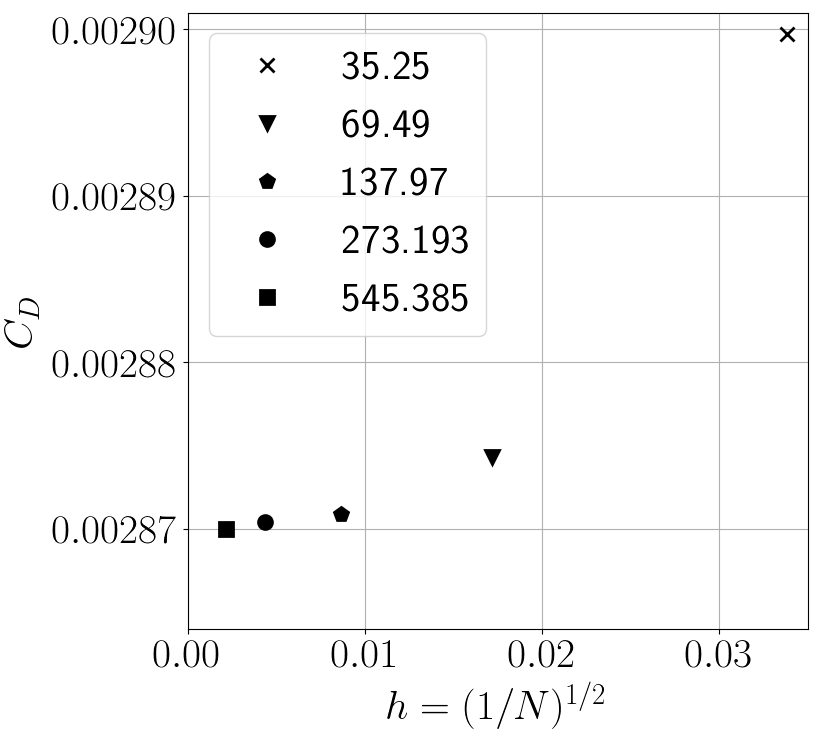
\includegraphics[width=1.\textwidth]{figures/FPconvstudy.png}
    \caption*{a) Integrated flat plate $C_D$}
  \end{minipage}
  \begin{minipage}{0.45\columnwidth}
  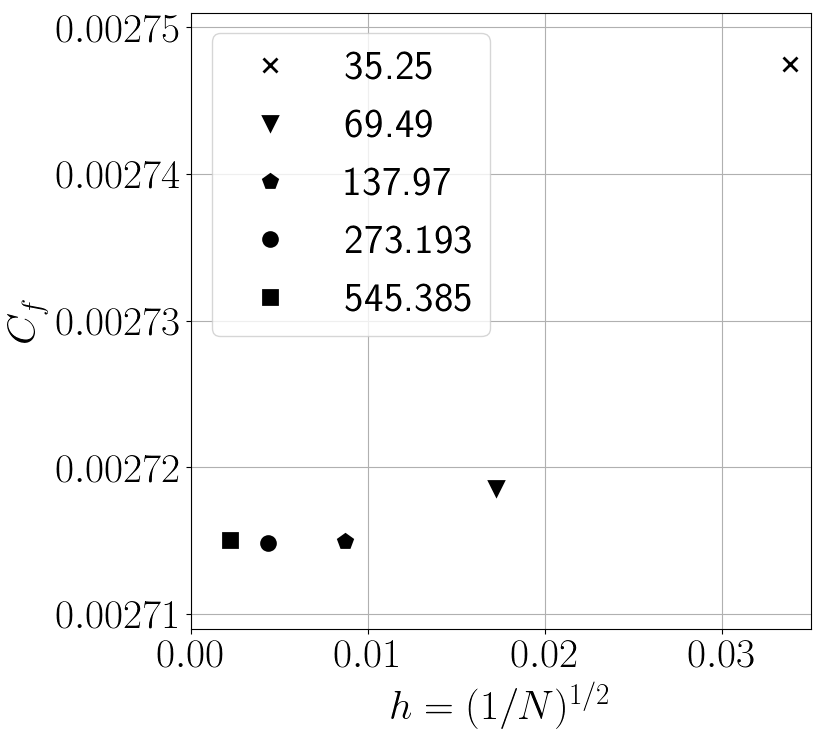
\includegraphics[width=1.\textwidth]{figures/FPconvstudyCF.png}
    \caption*{b) Local $C_f$ at $x=0.97$}
  \end{minipage}
  \caption{Mesh dependency study for the flat plate boundary layer build up.} \label{fig:FPconstudy}
\end{figure}
In Figure \ref{fig:FPCF} the skin friction coefficient, Eq. \ref{eq:CF}, is compared for the two solvers over the entire flat plate using Grid5. The two solvers agree well but as discussed before, due to the singularity point, the two solvers predict a different value at the leading edge. That means if one grid has a cell closer to the leading edge the value of $C_f$ would be higher, which causes the behavior seen in the figure.
\begin{figure}[H]
  \centering
  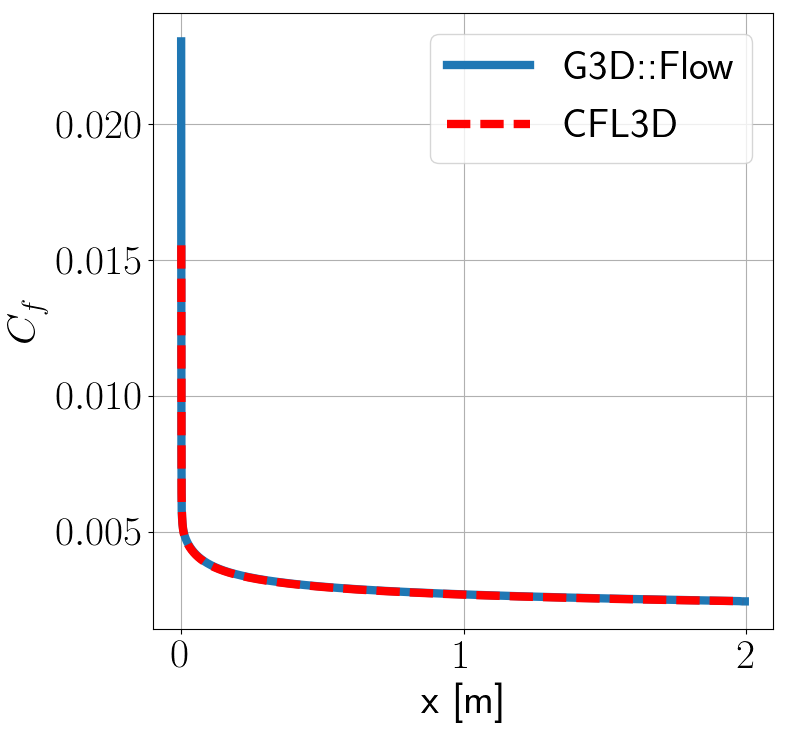
\includegraphics[width=0.5\textwidth]{figures/FPCF.png}
  \caption{Skin friction coefficient.} \label{fig:FPCF}
\end{figure}

In Figure \ref{fig:FPvel} the velocity profiles for the different solvers are compared at two different locations on the flat plate, at $x=0.97$ and $x=1.90$. The velocities are normalized with the free-stream velocity. As seen in the figure, which is limited in $y$-direction for better view of the near wall behaviour, the velocities are the same for the two solvers at both locations. 

In terms of the skin friction coefficient and velocity profiles the two solvers show almost identical results, where the only difference is due to a finer grid at the leading edge for the G3D::Flow solver. From these results it can be concluded that the G3D::Flow solver was successful in reproducing the results obtained by CFL3D when simulating a flat plate boundary layer build up using the SA turbulence model.
\begin{figure}[H]
  \centering
  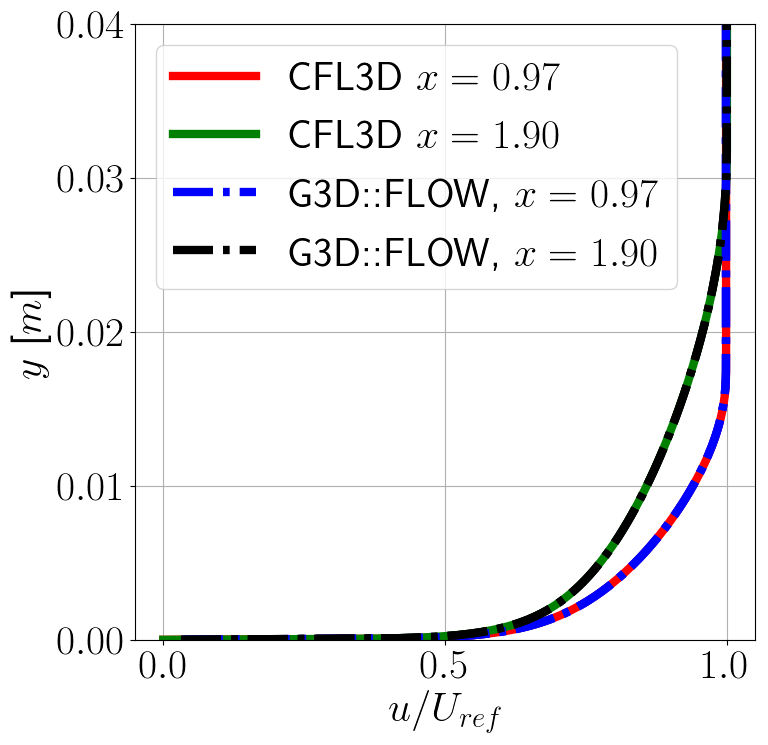
\includegraphics[width=0.5\textwidth]{figures/FPVelComp.png}
  \caption{Velocity profiles for $x=0.97$ and $x=1.90$.} \label{fig:FPvel}
\end{figure}

\section{Backward facing step\label{ch:BFS}}
Figure \ref{fig:BFS} presents the 2D BFS's computational setup where the boundary conditions are defined as well as the measures of the domain. The size of the domain is scaled with the step height ($H=0.0127m$).
\begin{figure}[h!]
  \centering
  \begin{tikzpicture}
\begin{axis}[
  axis x line=bottom,
  axis y line=left,
%  scale only axis,
  xtick={-150,-100,...,80},
  ytick={-1,0,2,...,10},
  xlabel={\bf{x [H]}},
  ylabel={\bf{y [H]}},
  xlabel style={below right},
  ylabel style={above left,rotate= -90},
  x=0.05cm,
  xmin=-150,
  xmax=80,
  ymin=-1,
  ymax=10]
\draw (40,100)--(20,100)--(20,20)--(40,20);
\draw[ultra thick] (40,20)--(150,20)--(150,10)--(200,10) (200,100)--(40,100);
  \draw (200,100)--(200,10);
%\draw[<->,very thick] (5,13)--(40,13);
\node at (80,60) {symmetry};
 \draw[-latex, very thick] (60,60)--(37,20);
 \draw[-latex,very thick] (60,60)--(37,100);
%\draw[<->,very thick] (40,13)--(240,13);
\node at (170,61) {visocus walls};
  \draw[-latex,very thick] (140,60)--(130,100);
  \draw[-latex,very thick] (140,60)--(130,20);
%\draw (40,10)--(40,17);
\node at (40,60) {inlet};
  \draw[latex-, very thick] (20,60)--(30,60);
\node at (220,61) {outlet};
  \draw[latex-, very thick] (200,61)--(208,61);
\node at (139,14.6) {H};
  \draw[latex-latex, very thick] (145,20)--(145,10);
  \draw (150,10)--(143,10);
\end{axis}
\end{tikzpicture}
  \caption{Computational domain for the backward facing step.}
  \label{fig:BFS}
\end{figure}
The boundary conditions for the BFS are shown in Table \ref{tab:BFSBC} where the inlet static pressure, temperature and SA viscosity are shown as well as the outlet static pressure. Both the temperature and pressure are given as a function of a reference variables where $T_{ref}=298$ and $p_{ref}=1atm$. The exit pressure is adjusted until the Mach number is approximately equal to 0.128 at $x/H=-4$. The Reynolds number based on the step height is $Re_H=36000$.
\begin{table}[H]
  \caption{Boundary conditions.} \label{tab:BFSBC}
  \vspace{2mm}
  \centering
\begin{tabular}{|c|c|c|c|c|}
  \hline
    & $p_{\ast}/p_{ref}$ & $T_{\ast}/T_{ref}$ & $ \tilde{\nu}$  \\
  \hlineB{2}
  Inlet   & $1.0$       & $1.0$ & $3\nu$ \\
  \hline
  Outlet  & $1.01$     & -     & - \\
  \hline
\end{tabular}
\end{table}
\subsection{Grid}
Three grids with different cell counts are used for the grid dependency study. The information for each grid can be seen in Table \ref{tab:BFSgrid}, where Grid1 is the coarsest one and Grid3 the finest. $n_x$ is the number of nodes in x direction, $n_{y1}$ is in the number of nodes in the y direction upstream of the step, $n_{y2}$ is the number of nodes in the y direction downstream of the step and $n_{tot}$ is the total number of nodes for each grid. The last column shows the average $y^+$ value of the first wall normal cells, averaged over the lower walls, upstream and downstream of the step, excluding the recirculation area downstream of the step and the symmetry at the inlet. The SA model is a low-Reynolds number model, as mentioned before, and therefore it is important to ensure that the $y^+$ value is smaller or equal to 1.0. This is satisfied for all grids.
\begin{table}[H]
  \caption{Grid information for the BFS.} \label{tab:BFSgrid}
  \vspace{2mm}
  \centering
\begin{tabular}{|c|r|r|r|r|c|}
  \hline
  Grid  & $n_x$ & $n_{y1}$ & $n_{y2}$ & $n_{tot}$  & $y^+$  \\
  \hlineB{2}
  Grid1   & 185& 65 & 114& 16778 & 0.60 \\
  \hline                 
  Grid2   & 369& 129& 226& 66322 & 0.15 \\
  \hline                 
  Grid3   & 740& 257& 450& 264485& 0.05 \\
  \hline
\end{tabular}
\end{table}
Figure \ref{fig:BFSgrid} shows Grid2, excluding major part of the domain upstream of the step. The cell sizes increase exponentially in the x-direction, from the step towards the outlet. In the y-direction, upstream of the step, the cell sizes increase exponentially towards the centre of the channel. This expands into the domain downstream of the step. The step itself is not resolved in the x-direction. For Grid2 the number of nodes are doubled compared to Grid1 whereas for Grid3 the number of nodes are doubled compared to Grid2.
\begin{figure}[H]
  \centering
\begin{tikzpicture}
  \node[anchor=south west,inner sep=0] at (0,0) {\includegraphics[width=0.8\textwidth, height=5cm]{figures/BFSmesh.pdf}};
  %\draw[help lines,step=.1] (0,0) grid (13,6);
\end{tikzpicture}
  \caption{The grid downstream of the step for Grid2.} \label{fig:BFSgrid}
\end{figure}

\subsection{Results}
A grid dependency study is performed to ensure that the solution is independent off the grid. The reattachment location, based on where the skin friction coefficient, Eq. \ref{eq:CF}, becomes positive after the step, is compared for the different grids. The comparison case performed by NASA, using the SA turbulence model \cite{NASA} is also included for reference. This comparison is presented in Figure \ref{fig:BFSconstudy} where the convergence is clear for the reattachment location.
\begin{figure}[H]
  \centering
  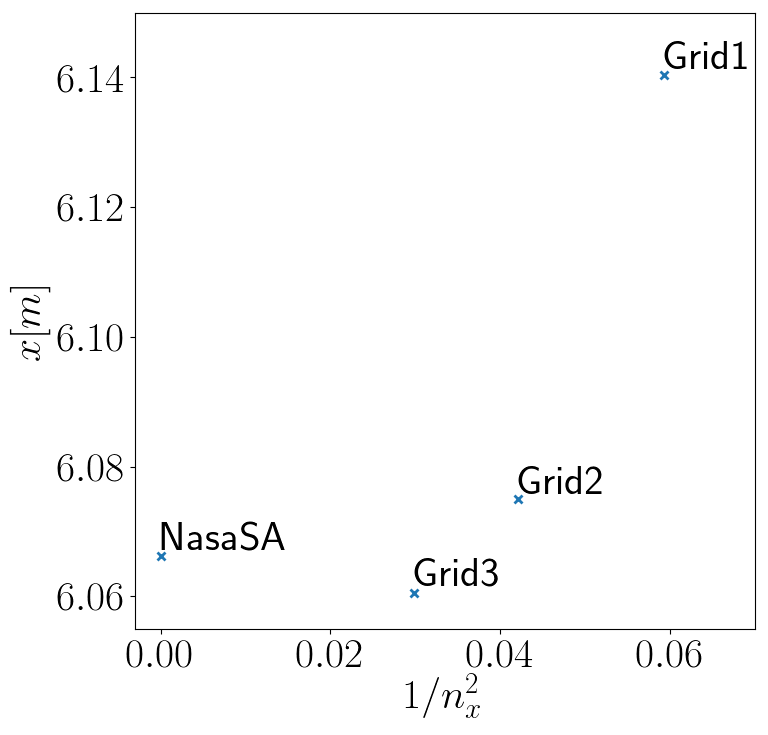
\includegraphics[width=0.5\textwidth]{figures/BFSAttachment.png}
  \caption{Mesh dependency study for the BFS.} \label{fig:BFSconstudy}
\end{figure}
The skin friction coefficient, Eq. \ref{eq:CF}, is compared in Figure \ref{fig:BFSCF}. As seen in the figure the two solvers agree very well. Overall the predictions are almost indistinguishable, with small differences just upstream and downstream of the step which might be a result of minor cell size differences in the flow-wise direction.
\begin{figure}[H]
  \centering
  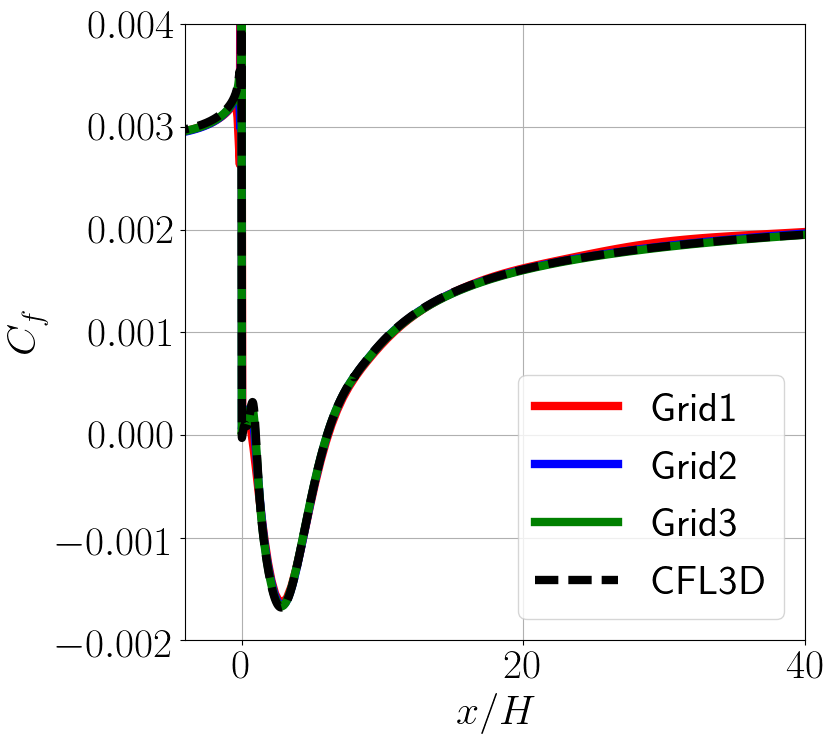
\includegraphics[width=0.5\textwidth]{figures/BFSCf.png}
  \caption{Skin friction coefficient.} \label{fig:BFSCF}
\end{figure}
In Figure \ref{fig:BFSCP} the pressure coefficient, Eq. \ref{eq:CP}, is shown. The data is shifted so $C_p=40$ at $x/H=40$. By analysing the figure it can be seen that the two solvers agree well, where minor difference is noticed at the step.
\begin{figure}[h!]
  \centering
  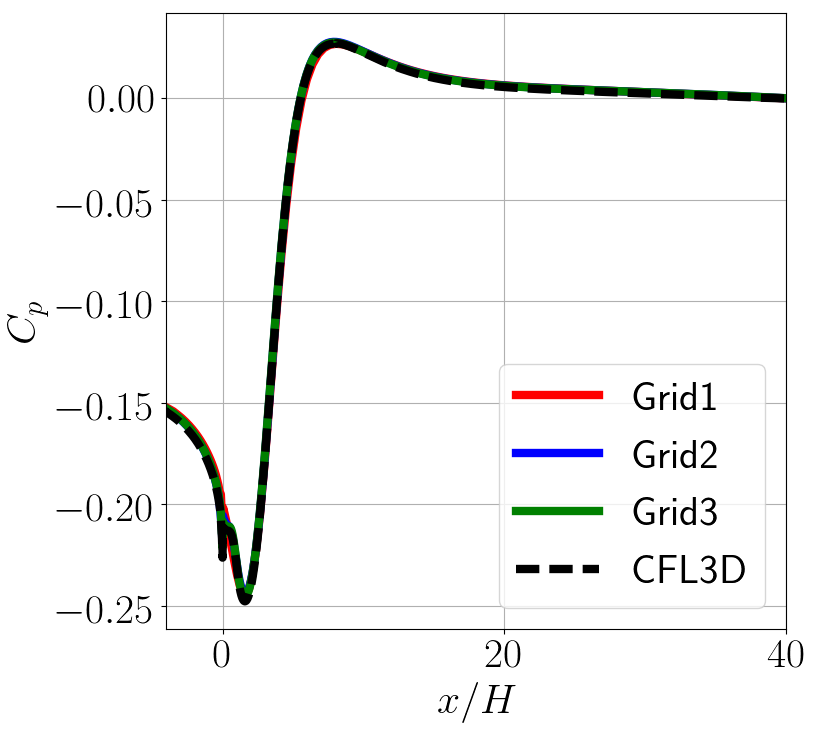
\includegraphics[width=0.5\textwidth]{figures/BFSCp.png}
  \caption{Pressure coefficient.} \label{fig:BFSCP}
\end{figure}

In Figure \ref{fig:BFSvel} the velocity profiles for 5 different x-locations are presented. The profiles are normalized with the maximum velocity at $x/H=-4$ and shifted dependent on each x-location, resulting in five velocity profiles at $x/H=\{-4,1,4,6,10\}$. As seen in the figure the two solvers are in a good agreement. 

\begin{figure}[h!]
  \centering
  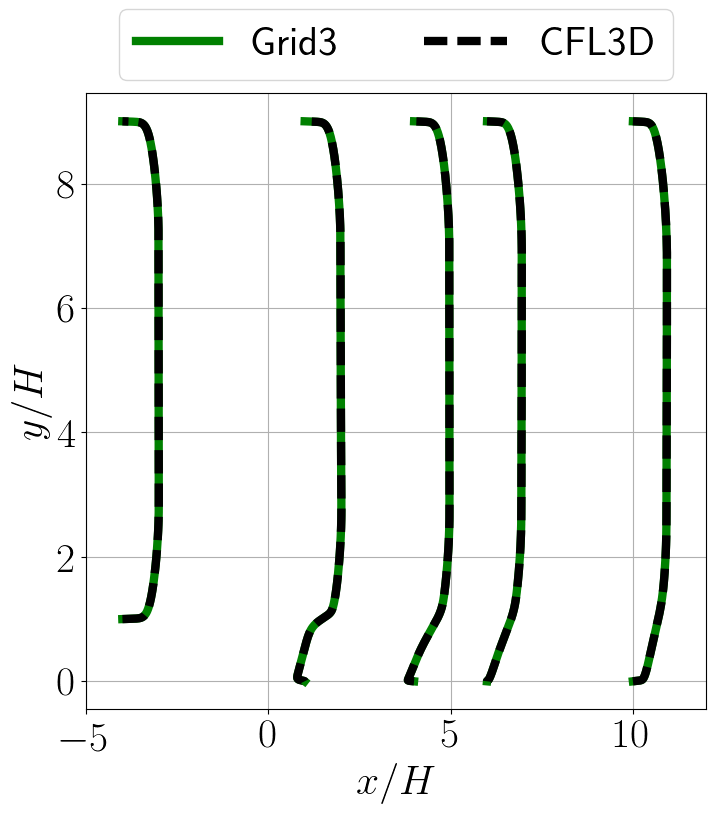
\includegraphics[width=0.5\textwidth]{figures/BFSVel.png}
  \caption{Velocity profiles at $x/H=-4$, $x/H=1$, $x/H=4$, $x/H=6$ and $x/H=10$.} \label{fig:BFSvel}
\end{figure}
\begin{figure}[h!]
  \centering
  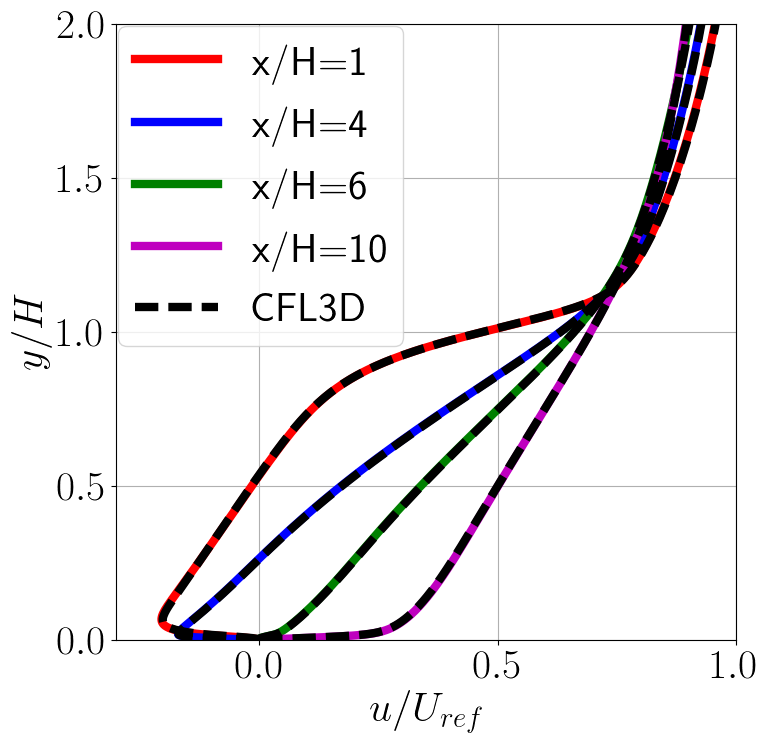
\includegraphics[width=0.5\textwidth]{figures/BFSVelBackStep.png}
  \caption{Zoom in on the velocity profiles downstream of the step at $x/H=1$, $x/H=4$, $x/H=6$ and $x/H=10$. The G3D::Flow simulations are performed using Grid3.} \label{fig:BFSvelBackStep}
\end{figure}
To be able to measure the performance of the G3D::Flow solver in more details, an enlarged figure of the velocity profiles behind the step is shown in Figure \ref{fig:BFSvelBackStep}. The same normalized velocity profiles are shown as before but without shifting the profiles to the corresponding x-location. Comparing the profiles it can be seen that the G3D::Flow solver is capable in reproducing the velocity profiles obtain using the CFL3D solver. 

In terms of the skin friction and pressure coefficients, as well as the velocity profiles, the two solvers give almost identical results where the main difference being at the step. That difference is insignificant and can be related to small differences is cell sizes. Furthermore the reattachment location downstream of the step compares well with the CFL3D location when considering the G3D::Flow Grid3 results. From these results it can be concluded that the G3D::Flow solver, using the SA turbulence model, is successful in simulating the BFS.
\section{Verification conclusion}
The SA turbulence model was implemented into the in-house code G3D::Flow. Two different verification cases were simulated and compared to a NASA \cite{NASA} database where in both cases the G3D::Flow solver was successful in reproducing the results obtained using the NASA CFL3D solver.
% 888888888888
% 88 
% 88
% 88
% 88
% 888888888888
%           88
%           88
%           88
%           88
% 888888888888
%           
%%%%%%%%%%%%%%%%%%%%%%%%%%%%%%%
%%%%%%%%%%%%%%%%%%%%%%%%%%%%%%%

\chapter{Concluding remarks\label{ch:conclusion}}
The following section presents the steps taken forward throughout this thesis to make it possible to simulate an ICD using the SA-DDES turbulence model.

The SA one-equation turbulence model was implemented into the Chalmers-developed in-house code G3D::Flow. The model implementation was verified by comparing it to results from a well-known CFD solver for simple test cases (Chapter \ref{ch:verification}). As the main objective was to run higher-fidelity models on the ICD, the SA-DDES model was implemented in the solver, where the SA model is used as an underlying SGS model and to solve the attached boundary layers.

As an initial step towards simulating the whole ICD experimental test rig with the DDES model, the configuration was simulated using the SA model and compared to experiments (\refpaper{B}) and the well-known CFX solver (Chapter \ref{ch:sim}). Comparing the G3D::Flow solver to experimental data and CFX, a good agreement was obtained, specially for the $10\%$ bleed fraction case. The higher bleed fraction had some convergence challenges due to pressure fluctuations, resulting in significant difference for the G3D::Flow results.

To analyse the performance of the DDES model a single PSW blade was ran in isolation (\refpaper{A}). This was done to minimize the computational cost while learning how the DDES model worked on a realistic and sufficiently complicated geometry. A literature study unveiled studies where the original DDES model coefficients where questioned and altered with good results. The lessons learned from those studies were applied to the study in \refpaper{A} with good results, even though the performance could be improved.

Simulating the PSW in time accurate mode, i.e. using global time-steps, means that a very low time-step must be used as the solver is fully explicit. This means that the smallest cells closest to the wall will dominate the maximum allowed time-step. Due to this the number of time-steps needed for a converged solution using the G3D::Flow solver is couple of orders of magnitude too high to be a realistic option.

\section{Future work}
To overcome the problem with small time-steps in the boundary layers different technique can be used where instead of calculating the boundary layer in RANS mode a wall-modelling methods can be applied. This is expected to perform similarly for attached flows, compared to the RANS resolved boundary layer, whereas for separated flows it will not be capable in predicted the flow as accurately. Both simulations and experiments showed no signs of major separation in the ICD and therefore the wall-modelling technique could be considered a reasonable option. There where however small separation areas at the trailing edges of the blade profiles which, if not captured, could result in different flow dynamics. The next step will be applying a wall-modelled RANS as underlying DDES model as it is relatively inexpensive compared to wall-modelled LES.

Taking a step forward in simulating interaction between real engine components, the stationary PSW is replaced by the last stage of the LPC, including both stator and rotor blades. This is expected to make the flow behaviour more complicated as the rotor blades wakes will pulsate onto the downstream components, instead of having a steady flow field. The difference compared to the current model will be analysed and evaluated in terms of computational cost and accuracy.


% 888888888888
% 88 
% 88
% 88
% 88
% 888888888888
% 88        88
% 88        88
% 88        88
% 88        88
% 888888888888
%           
%%%%%%%%%%%%%%%%%%%%%%%%%%%%%%%
%%%%%%%%%%%%%%%%%%%%%%%%%%%%%%%
\chapter{Summary of papers\label{ch:summary}}

\section{Paper A} \fullcite{MinSciTech18}
\subsection{Division of work}
Besides being the main author, my work consisted of grid generation, CFD simulations, post-processing and analysing the results. Co-authors supervised the work and provided feedback on the analysed results as well as providing the geometry.
\subsection{Summary and discussion}
In this paper, different versions of the DDES shielding function were applied to a single PSW blade with the objective to analyse the performance difference. Initially, too low boundary layer protection was encountered using the original DDES model. Due to this, an investigation in the sensitivity to different coefficients in the shielding function, which were calibrated using a flat plate simulation, was carried out. The coefficient was increase by a factor of two, resulting in better shielding performance. The performance was however not ideal as for the suction side of the blade the shielding function extended far outside the boundary layer. It was pointed out, during the presentation of this work, that this might be caused by the fact that the turbulent intensity at the inlet boundary condition was very low. It was also pointed out that the inlet boundary condition might need synthetic turbulence to maintain continuous transition from the modelled turbulent stresses inside the RANS region towards the resolved stresses in the LES region. These suggestions will be investigated further.


\section{Paper B} \fullcite{MinTurbo18}
\subsection{Division of work}
Besides being the main author, my work consisted of grid generation, CFD simulations, post-processing and analysing the results. Co-authors supervised the work and provided feedback on the analysed results as well as providing the geometry and the experimental data.
\subsection{Summary and discussion}
In this paper, the full experimental test was simulated. A comparison was made between the G3D::Flow solver and experimental data at two operating points, where $10\%$ and $30\%$ if the total inlet mass-flow was extracted through a bleed pipe upstream of the OGV. The SA one equation turbulence RANS model was used for the CFD simulations. For the lower bleed fraction case, the simulations agreed well with the experimental data in the ICD whereas for the higher bleed fraction case the simulations showed signs of strong instabilities, effecting the convergence of the solution. The reason for those instabilities was assumed to be caused by the short bleed pipe, resulting in strong effects from the bleed pipe outlet boundary condition. This showed that the bleed pipe needed to be extended for future simulations using higher bleed fractions.

Further investigations, conducted after the submission of the final paper, showed that even though with an extended bleed pipe the pressure instabilities persisted. With the extended bleed pipe, the solution became more stable where the flow was not blocked by the separated flow caused by the short bleed pipe. However, the bleed module's mesh was found to generate strong pressure fluctuations. Therefore, a new mesh was created, including the bleed pipe extension as well as an improved mesh of the whole module. The comparison of the two meshes is presented in Figure \ref{fig:BleedComp} where the improved one is shown to the left whereas the original is to the right. The main difference between the two meshes is the extension of the pipe (see Figure \ref{fig:bleed} for the whole module), increased number of cells in the axial direction and smoothening of cells in the area between the bleed pipe splitter and the domain inlet. These changes made the solution converge and the pressure fluctuations to disappear. The procedure used when generating the improved mesh will be used for future simulations.
\begin{figure}[H]
  \centering
  \begin{minipage}{0.49\columnwidth}
  \includegraphics[width=8.05cm, height=6cm]{figures/BleedGrid2DBM.pdf}
  \end{minipage}
  \begin{minipage}{0.49\columnwidth}
  \includegraphics[width=8.05cm, height=6cm]{figures/BleedGrid2DShort.pdf}
  \end{minipage}
    \caption{Comparison between the improved mesh (left) and the original (right).}\label{fig:BleedComp}
\end{figure}

%%%%%%%%%%%%%%%%%%%%%%%%%%%%%%%


